\documentclass[letterpaper,twocolumn,10pt]{sig-alternate-10pt}
%\documentclass[]{sig}
\usepackage{times}
\usepackage{graphicx}
\usepackage{mathtools}
\usepackage{amsmath}
\usepackage[utf8]{inputenc}
\usepackage{cleveref}
\usepackage{listings}
\usepackage{array}
\usepackage{breqn}
\usepackage{tikz}
\usepackage{algorithmicx}
\usepackage[Algorithm,ruled]{algorithm}
\usepackage{algpseudocode}
\usepackage{pifont,xspace}
\usetikzlibrary{automata,positioning}
\newcommand{\name}{Genesis\xspace}
\newcommand{\Name}{\name}
\newcommand{\pushcode}[1][1]{\hskip\dimexpr#1\algorithmicindent\relax}
\newcolumntype{P}[1]{>{\centering\arraybackslash}p{#1}}

\usepackage{caption}
\usepackage{enumitem}
%\usepackage{usenix}
\usepackage{epsfig}
%\usepackage[TABBOTCAP]{subfigure}
\usepackage{color}
%\usepackage{thumbpdf}
\usepackage{verbatim}
%\usepackage{hyperref}
\usepackage{url}
%\usepackage{booktabs}
\usepackage{colortbl}
\usepackage{enumitem}
\usepackage[export]{adjustbox}
\usepackage{subfig}
\newcommand{\minisection}[1]{\smallskip\noindent{\bf #1.}}
\newcommand{\secref}[1]{{\S\ref{#1}}}
\newcommand{\secsref}[2]{{Sections~\ref{#1} and \S\ref{#2}}}
\newcommand{\figref}[1]{{Figure~\ref{#1}}}
\newcommand{\figsref}[2]{{Figure~\ref{#1} and \ref{#2}}}
\newcommand{\appref}[1]{{Appendix~\ref{#1}}}
\newcommand{\thmref}[1]{{Theorem~\ref{#1}}}
\newcommand{\lemref}[1]{{Lemma~\ref{#1}}}
\newcommand{\corref}[1]{{Corollary~\ref{#1}}}
\newcommand{\proref}[1]{{Property~\ref{#1}}}
\newcommand{\tabref}[1]{{Table~\ref{#1}}}


\newcommand{\compactcaption}[1]{\vspace{-1em}\caption{#1}\vspace{-1em}}
\newcommand{\botcompactcaption}[1]{\caption{#1}\vspace{-1em}}
\newcommand{\topcompactcaption}[1]{\vspace{-1em}\caption{#1}\vspace{-0.5em}}

\newenvironment{compactitemize}
{
   \begin{itemize}[leftmargin=1.5em]
   \vspace{-1ex}
   \setlength{\topsep}{0pt}
   \setlength{\itemsep}{0em}
   \setlength{\parskip}{0pt}
   \setlength{\parsep}{0pt}
}
{
   \vspace{-1ex}
   \end{itemize}
}
\newenvironment{compact2itemize}
{
	\begin{itemize}[leftmargin=1.5em]
		\vspace{-1ex}
		\setlength{\topsep}{0pt}
		\setlength{\itemsep}{0.5em}
		\setlength{\parskip}{0pt}
		\setlength{\parsep}{0pt}
	}
	{
		\vspace{-1ex}
	\end{itemize}
}


\newenvironment{compactenumerate}
{
   \begin{enumerate}[leftmargin=1.5em]
   \vspace{-1ex}
   \setlength{\topsep}{0pt}
   \setlength{\itemsep}{0em}
   \setlength{\parskip}{0pt}
   \setlength{\parsep}{0pt}
}
{
   \vspace{-1ex}
   \end{enumerate}
}

%\usepackage[small,compact]{titlesec}
%\usepackage[font={bf,small}]{caption}

\newtheorem{mydef}{Definition}
\lstset{
	basicstyle=\itshape,
	xleftmargin=2em,
	literate={->}{$\rightarrow$}{2}
	{α}{$\alpha$}{1}
	{δ}{$\delta$}{1}
}


\crefname{section}{§}{§§}
\Crefname{section}{§}{§§}


\usepackage{color}
\newcommand{\loris}[1]{\textcolor[rgb]{0.00,0.00,1.00}{L: #1}}
\newcommand{\aditya}[1]{\textcolor[rgb]{0.00,0.00,1.00}{A:#1}}
\newcommand{\kausik}[1]{\textcolor[rgb]{0.00,1.00,0.00}{K: #1}}
\renewcommand{\aditya}[1]{{\color{red}{\bf AA: #1}}}

\usepackage{float}
%opening
\title{Genesis: Switch Table Synthesis for Policy Enforcement in Multi-tenant Networks}
\author{Paper \#107, XXX pages}
%\author{Kausik Subramanian, Loris D'Antoni, Aditya Akella \\
	%University of Wisconsin-Madison}

\begin{document}

\maketitle

\begin{abstract}
Operators of modern networks
require support for diverse and complex end-to-end policies, such
as, middlebox traversals, isolation, and traffic engineering. While 
Software-defined Networking (SDN) provides centralized 
custom routing functionality
in networks to realize these policies, many networks deploy "traditional"
control planes running distributed routing protocols like OSPF and BGP
because they are scalable and robust to failures. However, realization of 
policies by distributed control plane configurations is manual and error-prone. 
We show that synthesizing policy-compliant control planes is a
challenging problem and  propose a two-phase 
architecture to automatically realize 
policy-compliant control planes. 
The first phase
uses prior work to synthesize paths that satisfy the policies pertaining to the data-plane and 
the second phase uses constraint solving and Monte Carlo  search to synthesize
a control plane that produces the paths synthesized in the first phase and also satisfies the policies pertaining to configurations. 
%This last phase combines forma synthesis l tconstraint solving, for determining 
%the edge weights to be used for OSPF and BGP routing
%and 
%Markov Chain Monte Carlo (MCMC) sampling to identify a good way to partition the graph into
%multiple routing domains.
We implement our techniques in a tool \name and show that \name can
synthesize configurations for real topologies with up to 125 routers.
\end{abstract}
\section{Introduction}

Network operators of enterprise and cloud datacenter networks deal
with thousands of flow groups traversing large number of heterogeneous
devices. With growing diversity of applications, need for security and
compliance, and the advent of cloud comouting, these flow groups may
be subject to increasingly complex policies. Cloud tenants or
enterprises require basic reachability between hosts/application, and
middlebox traversal for certain flow groups. Operators, on top of that
require support for policies like traffic isolation between flows to
provide security and fairness, and satisfying resource constraints
pertaining link bandwidths and switch table sizes to perform traffic
engineering and network resource management.  However, configuring
network devices to implement these diverse and complex policies is
manual, ad-hoc and error prone today, leading to violations of
service-level agreements and mis-configurations which have severe
performance and security impacts.

%%  However, in real-life, the
%% process of policy enforcement by network operators is manual and
%% ad-hoc, leading to violations of service-level agreements and
%% mis-configurations which have severe performance and security
%% impacts. With the boom in cloud services, datacenter networks deal
%% with thousands of flows which are not constant, but in flux, thus,
%% making it difficult to enforce them in an ad-hoc manner.

%% Network operators desire various different end-to-end policies to
%% support in clouds and enterprise networks. Tenants or organisations
%% require support for basic policies like reachability between hosts,
%% and specifying different middlebox policies for certain
%% flows. Operators, on top of that require support for complex policies
%% like traffic isolation between flows to provide fairness and
%% specifying resource constraints like link bandwidth and switch table
%% sizes to perform traffic engineering and network resource management.

Though Software-defined Networking (SDN) has allowed network operators
to program networks in a more intuitive manner, many of existing SDN
tools/frameworks are too low-level in their functionality. Supporting
the aforementioned types of policies simply using SDN-capable switches
or with existing languages like Frenetic~\cite{frenetic} and
Pyretic~\cite{pyretic} is extremely challenging; operators would
ideally want to specify and realize policies network-wide without
programming individual switch behaviors. \aditya{we need to be careful
  not to bin all SDN languages into this switch-by-switch model}.
There has been research in the field of network-wide policy
enforcement in networks, like bandwidth provisioning in Merlin
\cite{Merlin}, and middlebox policy enforcement in SIMPLE
\cite{simple} or FlowTags~\cite{flowtags}. However, these approaches
are tailor-made to specific policies, and thus, difficult to extend it
to support other kinds of policies.

In this paper, we seek a {\em general} approach, where operators can
specify a variety of custom policies in a simple, declarative way, and
the complexities of correctly realizing the policies in the data plane
are hidden away from them. %% To support a cornucopia of policies, an
%% important feature is \emph{generality} of the approach of policy
%% enforcement, so that it can be extended to enforce custom policies
%% required by the operator.
By designing and implementing a system called \Name, this paper makes
a case for using \emph{efficient synthesis} of switch table forward
rules to realize this vision.
%% switch
%% table forwarding rules to the solve the problem of policy enforcement
%% by use of off-the-shelf SMT-solvers.

We show that enforcement of several of the policies supported by
\Name, specifically isolation, and middlebox traversal is
NP-complete. Thus, \Name leverages recent advances in creating fast
SMT solvers (e.g., Z3~\cite{z3}) to perform synthesis by encoding the
policy enforcement problem to a SMT instance, and using the SMT solver
to search for a solution, which is then translated into switch
rules. %% This paper presents Genesis, a
%% network management tool where the network operators can express the
%% network-wide policies in a high-level declarative manner and Genesis
%% will synthesize the lower-level switch forwarding rules for realising
%% these policies, eliminating the need for operators to work on
%% switch-level behaviours.
By leveraging a formal reasoning technique of SAT/SMT solving, \Name
eliminates the room for error in policy enforcement.

Unfortunately, naive application of SMT solvers results in synthesis
speeds that don't match the scale of operations of cloud and
enterprise networks today. \aditya{give an example as to how slow
  things can get} To overcome this challenge, \Name leverages a few
domain-specific ideas.  Specifically, it uses a novel search strategy
using regular expressions to prune the space of forwarding plane
configurations by leveraging data center network
structure. \aditya{the previous sentence is vague} knowlegde. Second,
\Name uses heuristical synthesis routine that leverages the nature of
policy interactions to improve synthesis performance. \aditya{quickly
  talk about in 1-2 sentences the speedup achieved with these
  optimizations}

%% are
%% huge, and by supporting a set of diverse and complex policies with
%% different search objectives, we require to create a model general and
%% expressive enough to support these. This poses a challenge as to can
%% synthesis performance be improved by leveraging knowledge specific to
%% the problem of policy enforcement in networks?

We implement \Name using ... We evaluate it using .... Key highlights .... \aditya{all of these are todo}.

Thus, the main contribution of this paper are: \aditya{todo}

%% : We present the design and implementation of a network management
%% system with support for a diverse set of complex end-to-end
%% policies like isolation, waypoints and capacity. We designed a
%% novel search strategy using regular expressions to prune the space
%% of forwarding plane configurations by leveraging the network
%% structure to provide properties of the path, especially in
%% datacenter topologies. Lastly, we design a heuristical synthesis
%% routine leveraging the nature of policy interactions to improve
%% synthesis performance.

\section{Motivation} \label{sec:motivation}
% Programming a legacy network control plane to satisfy a variety of
% connectivity, security, and performance policies is a complex and error-prone
% task. We have shown that program synthesis is a promising approach to automate
% this process and produce a control plane that is ``correct-by-construction.''
% In particular, we presented an architecture where a network operator provides
% a policy-compliant data plane and a set of hard and soft policies as input,
% and the system automatically provides a set of device configurations that
% leverage the control plane features available on each device to compute
% policy-compliant paths, even in the presence of failures.  Formulating a
% tractable synthesis problem and maximizing the number of satisfied soft
% policies are the key challenges in realizing this vision. We show these
% challenges can be overcome by modeling the control plane using a graph-based 
% abstract representation tied to a traditional shortest path algorithm and
% iteratively transforming the abstract representation based on feedback from
% the satisfiability (SAT) solver and characteristics of the graph. However, we
% have only explored how to address a subset of important policies and leverage a
% few available control plane features on traditional networking hardware. Our
% future work will focus on satisfying a wider range of policies using more
% features, and we will study how to best translate our abstract representation
% into actual device configurations to make our system practical for use with
% real networks.

One of the foremost tasks in network management is programming the network to
forward traffic in a manner consistent with user- and application-induced
policies. Common types of policies include: reachability (i.e., which
end-hosts can communicate), isolation (i.e., which flows cannot share links),
service chaining (i.e., which middleboxes must be traversed), resilience
(e.g., how many backup paths are available), and traffic engineering 
objectives like minimizing the average link utilization. Every
set of forwarding paths (i.e., data plane) installed in the network
%---either manually or by a control plane---
should conform to these 
policies, otherwise performance, security, or availability problems may arise.

% A variety of techniques can be used to determine the appropriate forwarding
% paths. One option is to compute a data plane offline, and install the data
% plane using an API that allows direct control of switches' forwarding tables
% (e.g., OpenFlow). Several recent works~\cite{merlin} have adopted this
% approach, using solvers to automatically compute a data
% plane that conforms to a set of policies. 
% A second option is to dynamically compute forwarding
% paths at a logically centralized controller---i.e., use a software-defined
% networking (SDN) control plane. However, this requires developing algorithms
% that take the set of policies and the current state of the network (e.g.,
% which links have failed) as input and output paths that conform to a
% multiplicity of policies.  Most existing SDN control applications only compute
% paths based on one or a few types of policies: e.g., service
% chaining~\cite{simple, flowtags}, traffic engineering~\cite{swan, b4}, or
% resilience~\cite{plinko}. Furthermore, in both approaches, the centralized policy
% component may become bottlenecked
% or fail (even if it is distributed), leading to (a partial) network failure.

A common theme among these policies is that 
they specify \emph{network-wide intent}~\cite{intent},
operators can specify what they \emph{want} from the network as a 
whole, instead of \emph{how} individual components of the network
must be configured. 
Software-defined networking (SDN) has led to the development 
of various frameworks for network-wide policy enforcement
~\cite{netkat, simple, merlin, fattire, genesis}. In SDN,
a centralized controller machine (control plane) controls
the end-to-end paths by managing forwarding rules on programmable
network switches (data plane). The controller can program
forwarding rules using the global view of the network
topology to meet application requirements. While SDN 
significantly enhances programmability of the network to 
satisfy the diverse policy requirements in multi-tenant
clouds and enterprise networks, it suffers from two 
major challenges: 
\emph{scalability} and \emph{failure-tolerance}. 

The centralized controller is responsible for installing 
forwarding rules to all switches, and thus, as network sizes
increase, the overhead of rule installation could increase
significantly. When a network failure (link/switch) occurs,
the controller has to detect and respond to the failure, and
even establishing connectivity between endpoints could be delayed.
Also, the controller is a central point of failure and controller
failure can lead to network disruptions. 
The principles of scalability and failure-tolerance 
were instrumental to the design
of 'traditional' networks (e.g., the Internet) using distributed
routing protocols like OSPF and BGP to manage forwarding in the 
network without a central control entity. Another reason for the 
slow adoption of SDN has been the cost involved in overhaul 
of the network with programmable switches.  

Unlike SDN which provide a clean abstraction
to program the network to satisfy policies 
on end-to-end paths,
programming (i.e., configuring) 
routers such that the paths computed by
the distributed routing protocols enforce the 
policies is challenging for several reasons: 
\setlist[itemize]{
    topsep=.5ex,
    itemsep=0ex,
    leftmargin=1em,
}
\begin{itemize}
%\setlength{\topsep}{0ex}
%\setlength{\itemsep}{0ex}
%\setlength{\parskip}{0pt}
%\setlength{\parsep}{0pt}
\item The available path-computation algorithms
available are predefined---e.g., OSPF uses
Dijkstra's shortest path---and their behavior can only be influenced
through a limited set of parameters---e.g.,
link weights. Similarly, BGP uses shortest
path routing at a domain-granularity, and have different
provisions to control routing (like local preferences).  
\item Operators can have 
heteregeneous protocol requirements based on operational
factors like scalability and cost, thus requiring to model
protocol interactions. 
\item Most policies are
global---i.e., they concern end-to-end paths, not individual devices and
links---making it difficult to map policies to
individual router configurations. 
\item Since failure-tolerance is handled in a distributed 
fashion with no involvement of a central control entity,  
failure-tolerance properties like resilience under bounded
number of network failures must be taken into account in
the generation of router configurations. 

%A single set of parameters must result in
%policy-compliant paths under all reasonable network states---e.g., a bounded
%number of link failures.
\end{itemize}

\begin{figure}
\centering
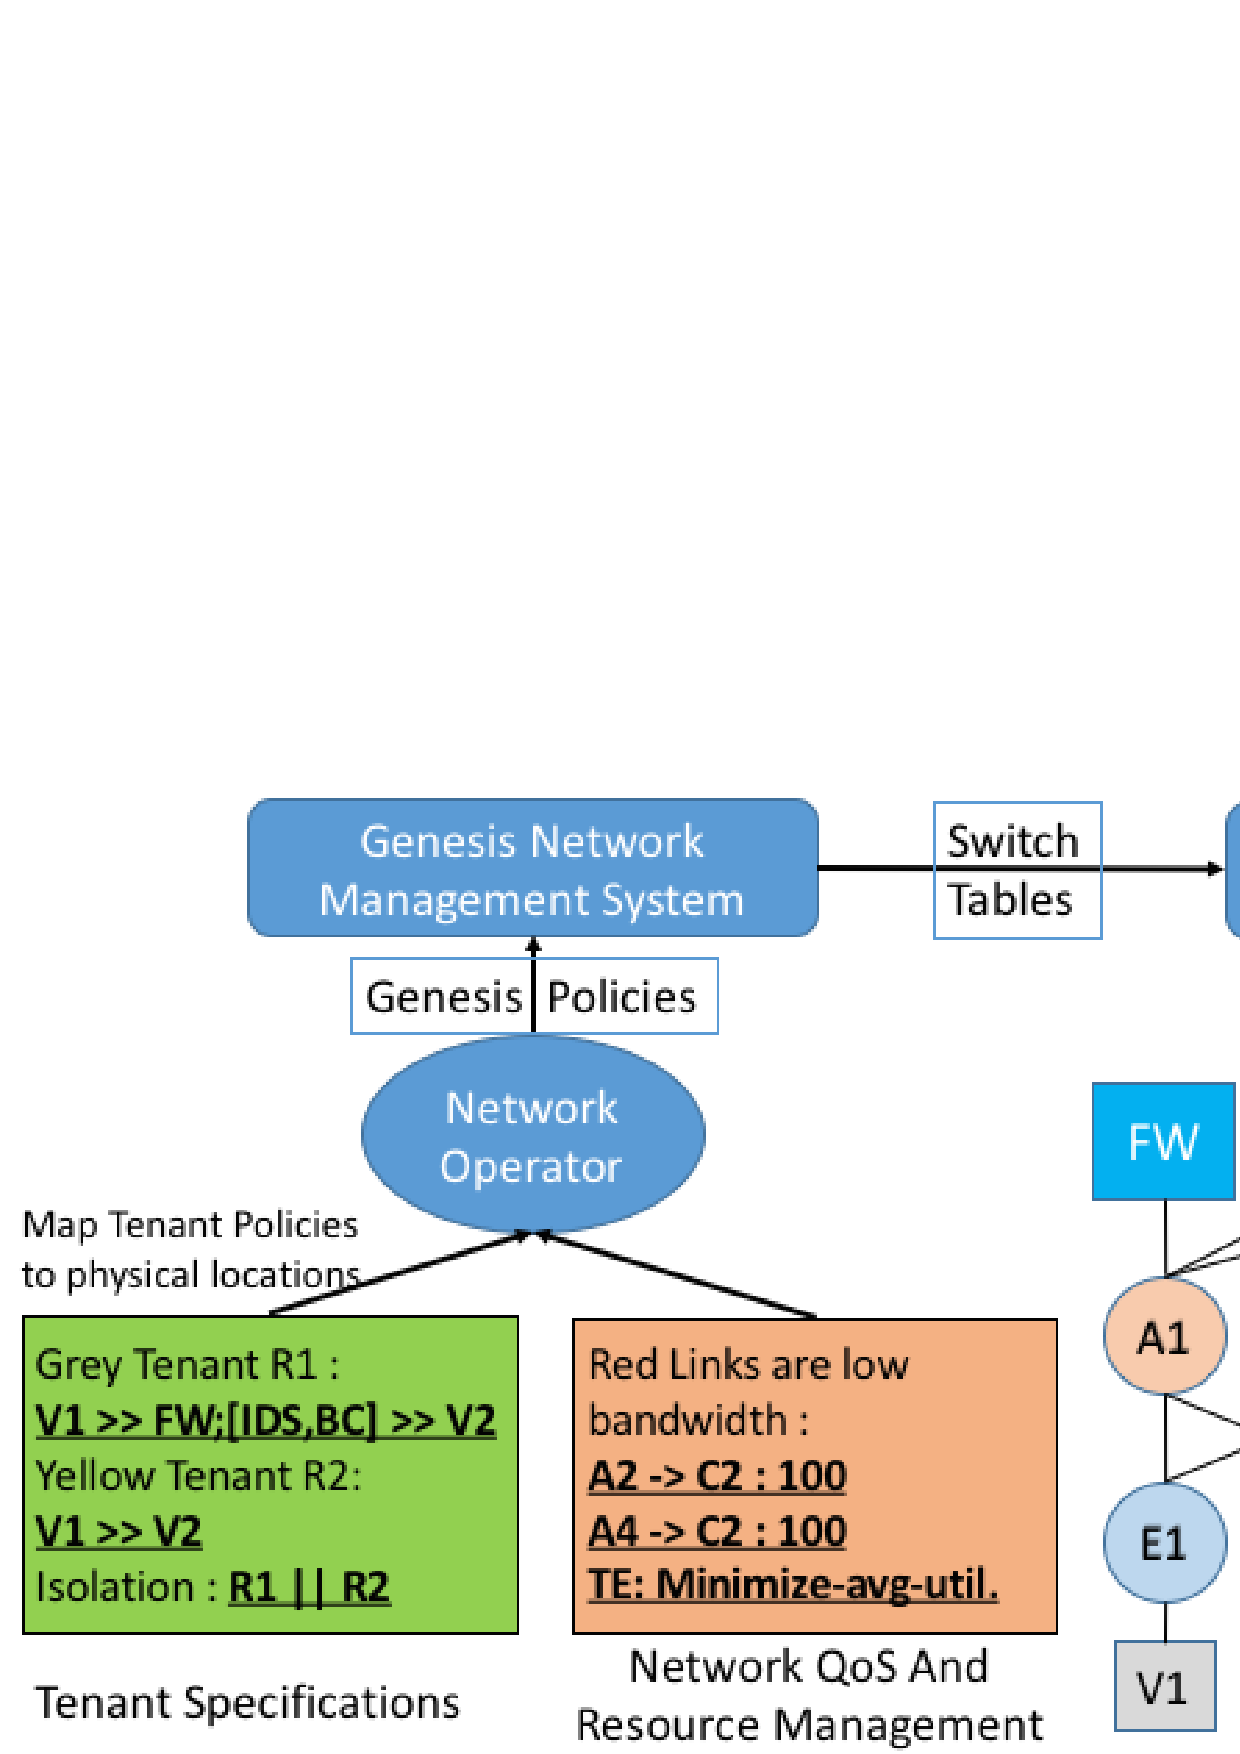
\includegraphics[width=\columnwidth]{figures/architecture.pdf}
\compactcaption{Two-phase process for generating a control plane
       with failure-tolerance properties}
\label{fig:architecture}
\end{figure}

\minisection{Configuration Synthesis}
To address the following challenges, we propose
\emph{automatic synthesis} of configurations, such that 
the network forwarding behaviour of the distributed
control plane meets policy specifications. 
Unfortunately, this task is inherently challenging 
as it requires solving in one shot multiple
computationally hard problems.
For example, even when considering 
static routing and no failures, 
synthesizing configurations 
that satisfy policies 
such as isolation and waypoints
is an NP-hard problem~\cite{genesis}.
Although the progress in SMT solving 
has made many NP-hard problems more practical, 
attempts of incorporating concepts such 
as shortest path algorithms 
into these solvers have resulted 
into huge performance losses~\cite{monosat}, 
not suited for real-world networks.

Our proposed approach is to tackle these problems 
in separate phases
(\figref{fig:architecture}).
First we synthesize a data plane that 
meets the input policies (\secref{sec:genesis}).
Using the data plane as input 
to the second phase, we 
express the problem of 
finding router configurations which 
induce the data plane provided by the
first phase using distributed routing
protocols (OSPF, BGP). Our contribution 
is \name, a framework for synthesizing
router configurations from the data
plane (paths) as input. 

\minisection{OSPF Synthesis}
For the OSPF protocol, configurations assign
weights to links between routers (directed edges
in the network topology). When the network has
to forward a packet from $s$ to $t$, the
OSPF routers uses 
Djikstra's algorithm to chose the
shortest weighted path from $s$ to $t$. Thus,
given input paths, \name finds edge weights 
(which are global for all paths) such that 
the shortest path through the network
for these endpoints exactly match the input paths. 
For example in \Cref{fig:ospfexample}(a), if the input
path is $s\rightarrow r_1 \rightarrow t$ for
destination IP $\lambda$, \name assigns
edge weights such that the input path has a strictly
smaller weight ($w=1+2$) than the other path $s \rightarrow t$ 
($w=5$). Thus, the OSPF routers will forward traffic for
$\lambda$ from $s$ to $t$ through $r_1$. \name 
efficiently computes weights by generating constraints
in the theory of Linear rational arithmetic (LRA) and
uses fast off-the-shelf LP Solvers 
(\secref{sec:ospfsynthesis}). 

However, given a set of paths as input, there may
not exist a solution to the edge weights. Consider the 
input paths as shown in \Cref{fig:ospfexample}(b). 
Both the red and blue paths are required 
to be the unique shortest path between $s$ to $t$
and, clearly, this is cannot be enforced for any 
choice of the edge weights (as weights correspond 
to all destinations). 
One way to synthesize configurations in this scenario 
is to ``disable'' the edge
$(s, t)$ for destination $\lambda_1$.
Using this technique, 
there is only one possible path from $s$ to $t$
for destination $\lambda_1$ ($s\rightarrow r_1 \rightarrow t$),
therefore is chosen as the shortest path. For 
destination $\lambda_2$, the $s\rightarrow t$ path
has a smaller weight ($w=1$) than the
$s\rightarrow r_1 \rightarrow t$ path ($w=1+2$), therefore,
both traffic is forwarded through the input paths for
both the destinations. 
This blocking mechanism is called a route-filter, and
we modify \name's OSPF synthesis algorithm to support
route-filtering (\secref{sec:filtering}).
 

\begin{figure}
	\centering
	\subfloat[Edge Weights]{
		\raisebox{0.5cm}{\resizebox {0.5\columnwidth} {!} {
	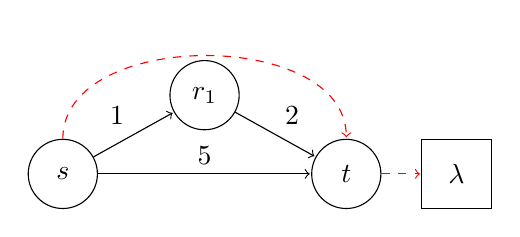
\begin{tikzpicture}[shorten >=0.5pt,node distance=,on grid,auto,
	square/.style={regular polygon,regular polygon sides=4}] 
	\node[state] at (0,0) (s)  {$s$}; 
	\node[state] at (1.8,1) (v1)  {$r_1$}; 
	\node[state] at (3.6, 0)(t) {$t$};
	\node[state, rectangle] at (5, 0) (d1) {$\lambda$};
	\path[->] 
	(s) edge node {1} (v1)
	edge  node {5} (t)
	edge [red, dashed, bend left=90] node {} (t)
	(v1) edge node {2} (t)
	(t) edge [red, dashed] node {} (d1);
	\end{tikzpicture}
	}}}
	\subfloat[Route-Filters]{
			\resizebox {0.5\columnwidth} {!} {
		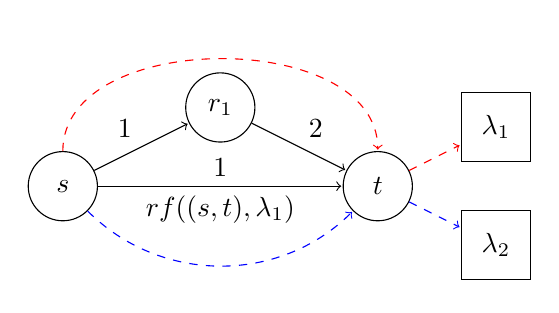
\begin{tikzpicture}[shorten >=0.5pt,node distance=,on grid,auto,
		square/.style={regular polygon,regular polygon sides=4}] 
		\node[state] at (0,0) (s)  {$s$}; 
		\node[state] at (2, 1) (v1)  {$r_1$}; 
		\node[state] at (4, 0)(t) {$t$};
		\node[state, rectangle] at (5.5, 0.75) (d1) {$\lambda_1$};
		\node[state, rectangle] at (5.5, -0.75) (d2) {$\lambda_2$};
		\path[->] 
		(s) edge node {1} (v1)
		edge  node [above] {1} node [below] {$rf((s,t),\lambda_1)$} (t)
		edge [red, dashed, bend left=90] node {} (t)
		edge [blue, dashed, bend right=45] node {} (t)
		(v1) edge node {2} (t)
		(t) edge [red, dashed] node {} (d1)
		(t) edge [blue, dashed] node {} (d2);
		\end{tikzpicture}
	}}
	\compactcaption{Example of paths which require route-filtering. This is a
		diamond starting at $s$ and ending at $t$. The diamond can be
		eliminated by filters $((s,r_1),\lambda_2)$ or $((s,r_2),\lambda_1)$.}
	\label{fig:ospfexample}
\end{figure}



\minisection{Dynamic Domain assignment}
The OSPF routing protocol does not scale 
with increasing network sizes
as it uses reliable
flooding of link-state packets. Flooding 
of updates can  
overwhelm the network when links fail. 
Ideally, operators would want to specify
limits on the size of an OSPF routing domain. 
Thus, a network could be 
split into multiple continuous OSPF domains,
which exchange routes across domains using
a inter-domain protocol like BGP.

We augment \name to synthesize 
inter-domain routing configurations 
such that each router is assigned to
a particular domain. 
Each domain is continous (all routers
are reachable to one another) and 
uses OSPF for intra-domain routing.
Domains exchange routes among  
themselves using BGP, a path-vector 
protocol which primarily selects routes by 
the number of domains in the route. 
However, \name can 
use BGP's powerful path selection metrics 
like local preferences such that  
paths with greater path lengths are selected.
OSPF has better convergence times than BGP,
thus, it is advantageous to use OSPF for 
routing in small domains and using BGP for
inter-domain routing. 

We consider the network to be managed by a 
single entity, therefore, the network can 
be split into domains\footnote{
The Internet is split into domains depending 
on ownership.} in numerous ways. Depending
on the network and input data plane, a certain
domain assignment of routers 
can optimize different metrics, like the
inter-domain configuration overhead (like BGP local
preferences and static routes) and OSPF route-filters
in the different domains. Thus, instead of operators
specifying a static domain assignment, \name stochastically
searches for the best domain assignment from the space of 
allowed assignments (for e.g., adhering to domain size limits)
to optimize different metrics. \name uses 
\emph{Markov chain Monte Carlo} sampling (MCMC) to perform
this stochastic search, and operators can specify parameters
to tune the cost function used in the search to assign priorities
to different metrics. 

\todo{Write about paper outline}





%ailures that happen in the later phases may require to restart the synthesis procedure 
%multiple times.
%but preliminary results of our approach are promising.


%The solution space of output network configurations to 
%enforce a set of policies
%is large; configurations can use different 
%network protocols (e.g., only BGP, only OSPF or a hybrid) and
%mechanisms (e.g., route filters, access control lists
%or protocol-specific variables). The large solution space
%of configurations complicates the synthesis of
%network configurations from
%input policies, 
%or ties the synthesis to a particular type of configuration. 
%Instead, we borrow a page from programming languages
%research and
%synthesize an Abstract Representation for Control planes (ARC)~\cite{arc} 
%from the data plane; the ARC can then be translated to actual device configurations.
%The ARC uses the notion that most routing protocols in use 
%today employ a cost-based path selection algorithm; thus a weighted
%graph can be used to abstractly represent the control plane such that 
%the path between two points taken in the network would be 
%the lowest weight path in the graph. 
%The ARC effectively decouples the policy component with the 
%actual network infrastructure. 

% While we use an abstract representation of the control
% plane (ARC) to simplify the synthesis, operators need control 
% planes conforming to certain requirements of the 
% underlying network infrastructure. For example, a 
% network may comprise of switches which do not have custom
% features like ACLs or route-filters, thus the ARC must take 
% into consideration these requirements. Without losing 
% generality, we translate these 
% requirements as types of ARCs with different properties,
% and still use a protocol-independent representation
% to represent the control plane. 

% In this paper, we primarily focus on 
% the second and third phase of our architecture, 
% i.e synthesizing a control plane from a set 
% of input paths and transforming the control plane to 
% satisfy policies under failure scenarios. The first 
% phase has seen promising work in recent times~\cite{merlin,
% simple}, these systems generate data planes to enforce 
% different kinds of policies, and 
% we can be retrofit these systems to generate different 
% data planes to integrate in our three-phase approach.

% thus, the networking infrastructure could be
% transitioned to different protocols without affecting the policy 
% control of the architecture. From the ARC, we can construct different
% drivers for translation to actual device configurations; these drivers
% can leverage inferences from healthy network practices in 
% real-life networks~\cite{mpa-imc15} to produce ideal network configurations.


%\aaron{Old text below}
%
%To tackle synthesis 
%of distributed control planes, 
%we use as input the network data plane 
%(set of forwarding paths) \aaron{Where does this data plane come from and
%    why is it reasonable to assume an operator can provide one?} which 
%enforces the operator-specified policies to
%synthesize an abstract representation of the control plane
%called ARC. \aaron{Our approach (ARC) should not come up until later in the
%    motivation, if at all.}
%The advantage of using network data planes as 
%input is the ease of developing
%different network management applications 
%enforcing proactive policies\footnote{
%Traditional control planes cannot support reactive policies, however
%middleboxes can overcome this limitation.} 
%as if operating over a software-defined
%network, agnostic of the actual network protocols used in the network.
%\aaron{I don't understand the preceding sentence. I'm still not clear why you
%take a single data plane as input and not multiple data planes or just the
%policies. I realize it is hard to synthesize from the latter, but can you be
%more precise why it is hard?}
%Many existing network management systems like Merlin~\cite{merlin} 
%and SIMPLE~\cite{simple}\footnote{
%Traditional control planes cannot support 
%paths with loops for service chaining.} developed for SDNs 
%could be seamlessly integrated to the architecture with minimal changes.
%\aaron{Do we need the preceding sentence?}
%Thus, using the data plane as input, we synthesize a control plane
%such that the paths decided by the control plane are the same 
%as the data plane input, and these paths satisfy the operator 
%policies.
%
%However, the control plane does not guarantee policy compliance 
%when failures occur. For
%example, if a link along the shortest path 
%%(\aaron{refer to some example figure}) 
%fails, \aaron{Need to mention earlier that we assume shortest-path-based route
%computations, ala OSPF} the next shortest path will become the new path to reach the
%destination. The control plane automatically computes the new shortest path
%(assuming one exists), thus preserving connectivity. 
%However, the new path may
%not conform to the same policies as the path in the 
%original failure-free data
%plane from which the control plane was synthesized: 
%e.g., the new path may no longer
%traverse a waypoint or have the same bandwidth capacity. Thus,
%synthesis must take into account policy-compliance under failures.
%
%Policy-compliance under failures is difficult to achieve due 
%to the large number of failure scenarios to consider and can 
%be impossible to synthesize a control plane which is 
%policy-compliant under all failures. Operators require 
%varying degrees of policy-compliance under failures for 
%which we propose two classes of policies: {\em hard} and
%{\em soft} policies. Operators can specify 
%hard policies pertaining
%to security are of the utmost importance, 
%because they protect the network and
%its services from attacks and unauthorized accesses. Some 
%examples of hard policies are as follows: 
%a particular flow must always traverse through a waypoint 
%under any failure scenario, or a certain pair of hosts must 
%never be able to communicate (always blocked). 
%Soft policies can be considered as objectives which improve 
%the control plane, but are not strict requirements, typically
%pertaining to performance. The consequences of violating
%soft policies are less severe. Operators can provide 
%backup paths for flows (generated such that they 
%satisfy the data plane policies) as soft policies, 
%and the synthesis of the control plane 
%tries to satisfy as many soft policies as 
%possible. 
%
%\aaron{Discussion of the available control plane constructs should come up
%    earlier.}
%While we use an abstract representation of the control
%plane (ARC) to simplify the synthesis, operators need control 
%planes conforming to certain requirements of the 
%underlying network infrastructure. For example, a 
%network may comprise of switches which do not have custom
%features like ACLs or route-filters, thus the ARC must take 
%into consideration these requirements. Without losing 
%generality, we translate these 
%requirements as policies determining the properties of the
%ARC, and thus, still use a protocol-independent representation
%to represent the control plane. 
%
%Our architecture envisions network operator providing
%a policy-compliant data plane and a set of hard and soft policies
%pertaining to policy-compliance under failure and network 
%infrastructure requirements as input to synthesize resilient 
%control planes. Towards this vision, we present  
%approaches to synthesize different types of the ARC and the 
%challenges involved in making synthesis efficient and
%extending these approaches to support a wider range of 
%policies and functionalities. 

\section{Control Plane Synthesis via ARCs} \label{sec:synthesis}
In this section, we describe preliminary ideas on how each phase of our synthesis 
approach can be implemented.
First, we briefly discuss how existing tools can be used to generate
policy-compliant paths (\secref{phase1}).
Second, we show how to generate ARCs that induce
the set of paths synthesized in the first phase (\secref{phase2}).
Third, we show how ARCs can be modified to deal with resilience (\secref{TODO}).
Finally, we show how to restart the process whenever one of the three phases fails (\secref{TODO}).

\subsection{From policies to paths} \label{sec:phase1}
The first phase of our approach produces a set of paths adhering to
different policies like reachability, service chaining, traffic engineering and isolation.
Synthesizing sets of paths---i.e., data planes---that adhere to a given set of policies
is already a hard problem, but a few practical approaches have been proposed.
The approach that is most similar to ours is the one used in Merlin~\cite{merlin}.
Given a set of waypoints, reachability, and bandwidth guarantee policies,
Merlin generates a mixed integer linear programming instance. 
A solution to this instance is a set of paths meeting the input policies.
Our prototype implementation uses a similar idea and,
since this part of the problem is not novel, we briefly provide the intuition behind our solution.
Given a set of policies we generate a set of constraints over the propositional theory of rationals 
and the solutions to these constraints are paths satisfying all the policies.
Our rich policy language requires complex Boolean reasoning that forces us to adopt propositional theories
in place of simple conjunctions of constraints.
In particular, policies like isolation and waypoints require disjunctive formulas.

%\loris{we will add more details if needed}


\subsection{From paths to ARCs} \label{sec:phase2}

The second phase of our approach takes as input the set of paths produced by the first phase
and produces an Abstract Representation of the Control Plane (ARC) that realizes the given set of paths.
First, we consider the problem of generating ARCs that
 forward packets based on shortest-paths---e.g., OSPF routing.
Then, we consider more complex forms of ARCs in which 
 additional mechanisms like route-filtering are allowed. 
 
\subsubsection{From paths to simplified ARCs}
The \emph{Simplified Abstract Representation of the Control Plane} (sARC) is a directed graph comprising switches as 
vertices and weighted edges corresponding to all links in the
topology. 
This is an ideal control plane supporting classic shortest path routing in which no links can be disabled. 

The problem of synthesizing 
a sARC that realizes an input set of paths reduces to a
variation of the so-called {\em inverse shortest path} problem~\cite{isp}. 
Assume we are given the following inputs: (1) a directed graph $T = (S, L)$ (the network topology), 
(2) a set of endpoints $\Gamma \subseteq S\times S$
describing the sources and destinations of the input paths, and 
(3) a function $P: \Gamma \rightarrow 2^{L^*}$
that assigns to each pair of endpoints $(s,t) \in \Gamma$ 
a set of \emph{acyclic} paths, such that for every path $l_0\cdots l_n\in P(s,t)$,
$l_0=(s,s')$, for some $s'\in S$, and $l_n=(s'',t)$, for some $s''\in S$.\footnote{
We use $L^*$ the denote the set of all finite sequences over the set $L$.}
The 
\emph{sARC synthesis}
problem is to find rational weights for the edges in $L$ such that 
for each pair of endpoints $(s,t) \in \Gamma$, 
the paths in $P(s,t)$ are \emph{the} shortest paths from $s$ to $t$ 
in the graph. Notice, that there can be multiple shortest
paths of equal cost for multi-path support (e.g., for traffic engineering).

In sARC, packet forwarding is based on destination.
For a destination $d$, we call $\xi_d$ the directed
subgraph of $T$ obtained by only keeping the nodes and edges 
that are traversed by paths with destination $d$.
Since paths are acyclic, $\xi_d$ is a directed acyclic graph.
We use $\Omega=\{d\mid (\_,d)\in\Gamma\}$ to denote the 
set of all destinations and $\Delta=\{\xi_d\mid d\in \Omega\}$ to denote  
the set of all destination DAGs. 

We use  $sw_1\rightarrow sw_2$ to denote $(sw_1,sw_2)\in L$ and
$sw_1\rightarrow^* sw_2$ (resp. $sw_1\rightarrow^+ sw_2$) to denote 
that $sw_2$ is reachable from $sw_1$ by crossing zero (resp. one) or more links in $T$.
Similarly, we use $\rightarrow_{\xi_d}$ to denote the same relations in the destination DAGs.


\minisection{Distance Equations}
To solve the sARC synthesis problem, we generate a set of linear equations
to find the required edge weights. 
We use $E(sw_1, sw_2)$ to denote the weight of the edge $(sw_1,sw_2)\in L$
and 
$D(sw_1, sw_2)$ to denote the shortest distance from $sw_1$ to $sw_2$.
We add the equation $D(s,s) = 0$ for every $s\in S$ to denote that the distance
from a node to itself is $0$.
The
following equation guarantees that $D(s,t)$ is not greater than 
the actual shortest distance from $s$ to $t$.
\begin{multline} \label{eq:dist}
\forall s, t, sw. (s \rightarrow sw \rightarrow^* t).\\
D(s, t) \leq E(s, sw) + D(sw, t)
\end{multline}

For each destination DAG $\xi_d\in\Delta$, we add equations to ensure 
that the input paths with destination $d$ are indeed the shortest ones.
 If a path
is the shortest path between its endpoints, then every 
subpath of the path has to be the shortest between its endpoints
as well (otherwise the complete path would not be the shortest).
\begin{figure}[h!] 
	\centering
	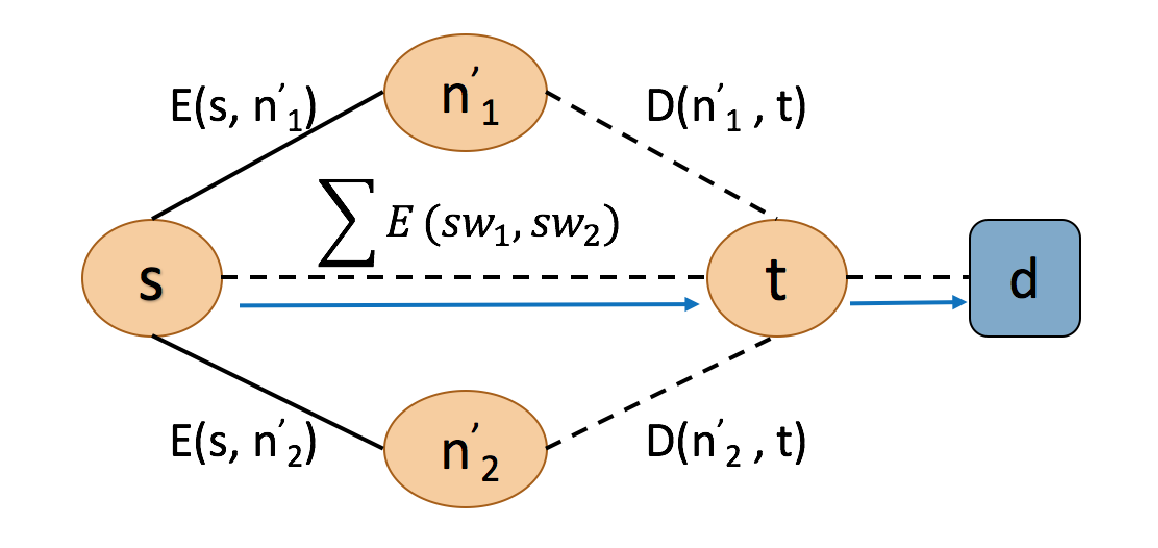
\includegraphics[width=0.8\columnwidth]{figures/distanceEquation.eps}
	\caption{An example illustration of the distance equations for shortest path forwarding.
		The pointed arrows represent the path in DAG of destination $d$, and the
		dotted line represents 1 or more edges. 
	} \label{fig:disteq}
\end{figure}
Consider a DAG $\xi_d$ for destination $d$. We define two neighbour
functions: $N_T(s)$ denotes the set of neighbours of switch $s$ 
in the input graph $T$, and $N_{\xi_d}(s)$ denote the set of
neighbours of switch $s$ in the destination DAG $\xi_d$. 
Given a destination $d\in \Omega$,
we use the following equations to ensure that, given two nodes $s$ and $t$ in
$\xi_d$, 
the set of paths from $s$ to $t$ in $\xi_d$ are
exactly
\emph{the} shortest paths from $s$ to $t$ in $T$ (\Cref{fig:disteq} illustrates 
an example).
Let $s,t$ be two nodes in $\xi_d$ and let  $Paths_{\xi_d}(s,t)$ be the set of paths from $s$ to $t$ in $\xi_d$.
\begin{multline} \label{eq:uniq1}
		\forall l_0\cdots l_n\in Paths_{\xi_d}(s,t).
		\forall n' \in N(s) \setminus N_{\xi_d}(s). \\
		E(s, n') + D(n', t) > \sum_{\mathclap{\substack{l_i=(s_i,t_i)}}} 
		E(s_i, t_i) 
\end{multline}
\begin{multline} \label{eq:uniq2}
		\forall l_0\cdots l_n\in Paths_{\xi_d}(s,t).
		\forall n' \in N_{\xi_d}(s). n' \not\rightarrow^+_{\xi_d} t.  \\
		E(s, n') + D(n', t) > \sum_{\mathclap{\substack{l_i=(s_i,t_i)}}} 
		E(s_i, t_i) 
\end{multline}
\begin{multline} \label{eq:uniq3}
		\forall l_0\cdots l_n, l_0'\cdots l_n'\in Paths_{\xi_d}(s,t).\\
		\sum_{\mathclap{\substack{l_i=(s_i,t_i)}}} 
		E(s_i, t_i)  =\sum_{\mathclap{\substack{l_i'=(s_i',t_i')}}} 
		E(s_i', t_i') 
\end{multline}
Equation~\ref{eq:uniq1} guarantees that 
the sum of the weights belonging to a path from $s$ to $t$ in $\xi_d$ is smaller than 
any path that goes to $t$ via a node $n'$ that is a neighbour of $s$ in $T$ but not in $\xi_d$.
Equation~\ref{eq:uniq2} guarantees that
the sum of the weights belonging to a path from $s$ to $t$ in $\xi_d$ is smaller than 
any path that goes to $t$ via a node $n'$ that is a neighbour of $s$ in $\xi_d$ but such that
$t$ is not reachable from $n'$ in $\xi_d$.
Finally, Equation~\ref{eq:uniq2} guarantees that all the paths from $s$ to $t$ in $\xi_d$ have the same weight.

% If the path $n' \rightarrow^* t$ 
% is not in any DAG completely, then
% $D(n',t)$ can be smaller than the actual shortest distance by the
% semantics of \Cref{eq:dist} (as
% $D(n',t)$ is not equal to any quantity by \Cref{eq:shortest}).
% However, since $D(n',t)$ is on the RHS of the equations in \Cref{eq:uniq},
% the equations will ensure that the path $s\rightarrow n \rightarrow^* t$
% has strictly greater weight than the path of the DAG.

%TODO: Add some figures

%- in some cases search is still hard but the network operator might have an idea of what the path patterns might or might not look like - Done
%- example? - Done
%- a good way to express this is to add extra constraints of the form ... - Done
%- we formally define a subset of regexes that...?
%- algorithm
%- brief comparison with netgen
\section{Tactics} \label{sec:tactic}
Synthesis for a reachability policy translates to choosing a path from the 
solution space of all paths from the source to destination such that the 
chosen path satisfies all policies like waypoints and isolation. Datacenter 
topologies like fat-trees~\cite{fattree} have numerous paths between 
edge switches to provide full bisection bandwidth. 
Thus, the solution space of paths for a pair of endpoints is large. 
For example, consider the fat-tree topology in \Cref{fig:fattree}. 
The number of paths under length 10 between two edge  switches 
in the same pod is 242 and two edge switches in different pods is 272. 
If we consider the synthesis of $n$ packet classes, the problem 
roughly translates to finding a solution in the space of size $n \times 242$.
\begin{figure}[h]
	\includegraphics[width=\columnwidth]{figures/fattree.png}
	\caption{Fat Tree Topology}
	\label{fig:fattree}
\end{figure}
Operators can leverage the network structure of topologies
 to reduce the solution space by specifying undesirable path patterns. 
 For example, a path from edge to edge in a fat-tree must not traverse another edge switch.
 This pattern will not drastically reduce the solution space of paths 
 due to the dense interconnect between aggregate and core switches,
 ensuring that synthesis most likely will not fail. 

We introduce \emph{tactics} (the name is inspired from the usage in SMT solvers, not 
proof assistants)
on labels, abstractions that allow the 
operator to impose a high-level restriction on the paths. 
We use the notion of mapping set of switches to labels to 
have a coarse-grained way for specifying path patterns. This helps
to create search strategies which can be used for majority 
of the packet classes instead of individual switch-level patterns which
lack generality.

 Let $Lb$ be the set of labels and $S$ be the set of switches in the topology. Let $\phi : S \rightarrow Lb$ be the labeling function that maps each switch to a label in $Lb$. One example for $\phi$ in the fat-tree topology in \Cref{fig:fattree} can be that we map all switches in the same level (core, aggregate or edge) to the same label,
therefore leveraging the hierarchical structure of the topology. A path $p$ is a word over the alphabet $S$. 
We define the path-labeling function $\Phi : S^* \rightarrow Lb^*$,  which maps each switch in the path to its corresponding 
 label. 
 For example, given the path $p = e1\ a2\ c3\ a4\ e2$, the path-labeling function function produces $\Phi(p) = eacae$ -- map each switch to its corresponding label.
 Here, $e$, $a$, and $c$ stand for edge, aggregate, and core respectively.

\subsection{Synthesis with Tactics}
%We use regular expressions and finite automaton to prune the constraints and impose restrictions on the path. The natural way for operators to specify tactics are using \emph{blacklists}, which specify what the path should not be. To express this in a intuitive manner, we use regular expressions on the set of labels to specify blacklists. For example, to blacklist paths from a edge switch to edge switch to not go through another edge switch, we can describe the tactic as $\neg (e .^* e .^* e)$ where the label of all edge switches is $e$. Another tactic is of the form $\neg (e (.)^4 a c .* e)$ which specifies we have a path of length 4, we do not go in the direction towards the core (as to reach the edge, the path would have to then go downwards from the core). 
Tactics are simple regular expressions over the set
 of labels and are used to blacklist certain path patterns.
Regular expressions have been previously used in tools like
NetGen~\cite{netgen} to specify the paths for the packet class.
While supporting full regular expressions is possible, it causes a blow-up in the solving time as further
constraints need to be added to the solver to ensure that the path satisfies the regular expression. 
%TODO \loris{is this true?}. % : Cross-check with Aditya. 
Instead, using the notion of switch labels, we use regular expressions to provide high-level path properties as a {\em search strategy} rather than a policy requirement. 
Instead of specifying how the path must look like, we use regular expressions on switch labels to specify \emph{blacklists}--i.e.,
what the path must \emph{not} look like. A tactic, for example, can blacklist paths from an edge switch to an edge switch that go through another edge switch. 
%\loris{we need a plot for the full regex thing to compare with Madhu, it would be great to repeat some of their experiments}

\subsubsection{Restricted tactic syntax} 
For specifying tactics, we identified a restricted set of regular expressions\footnote{
	It is a subset of star-free languages~\cite{starfree}.}
 that not only do not require extra constraints to be added,
but actually allow us to reduce the number of constraints. 
This set is defined using the following grammar:
$$\begin{array}{rcl}
R  &  :=  &  \neg (l_{src} .^i C .^* l_{dst}) \\
C  &  :=  &  \varepsilon \mid l_1 \mid l_1 l_2\\
\end{array}$$
where $l_i\in Lb$ and $l_{src}, l_{dst}$ are used to specify the labels of the source switch 
and destination switch, respectively, of the packet classes to which we apply the tactic. 
Since our goal is to black-list paths, we allow regular expressions to be negated at the outer level. 
\begin{example}
 $\neg (e .^i c .^* e)$ says that the path must not contain an core a switch at the $(i+1)^{th}$ step. 
 Similarly, $\neg (e .^i .^* e)$ says that the path connecting two edge switches should have a length $ < i + 1$. 
\end{example}


Let $\pi = sw_0\ldots sw_k$ be a path for packet class $pc$
and let its labeling be $\Phi(\pi)= a_0\ldots a_k$.
We say that $\pi$ satisfies a tactic $R$,  $\Phi(\pi) \in L(R)$, if the following
holds:
\begin{compact2itemize}
\item $\Phi(\pi) \in L(\neg R)$ iff $\Phi(\pi) \not\in L(R)$;
\item $\Phi(\pi) \in L( l_{src} .^i .^* l_{dst})$ iff $k\geq i+1$, $l_{src}= a_0$, and $l_{dst}= a_k$; 
\item $\Phi(\pi)  \in L (l_{src} .^i l.^* l_{dst})$ iff $k\geq i+2$, $l_{src}= a_0$, $l_{dst}= a_k$, and $a_{i+1}=l$;
\item $\Phi(\pi)  \in L( l_{src} .^i l_1 l_2.^* l_{dst})$ iff $k\geq i+3$, $l_{src}= a_0$, $l_{dst}= a_k$, $a_{i+1}=l_1$, and $a_{i+2}=l_2$.
\end{compact2itemize}
In \Name, operators can specify conjunctions of tactics which adhere to the restricted 
syntax and the synthesis algorithm is modified to enforce the tactics. 
Since tactics are path-related restrictions, 
operators can also apply tactics selectively to the paths for certain packet classes, and also different tactics for different classes. 
\begin{example}
A complex form of tactic which ensures that a edge-edge path
cannot traverse another edge switch can be expressed using conjunctions:
$\neg (e .^* e .^* e)\equiv \bigwedge \limits_{i=0}^{i=\mu-2} \neg (e .^i e .^* e)$ where $\mu$ is the synthetic limit on path length. 
\end{example}


\subsubsection{Modified Synthesis Algorithm with Tactics}
In our synthesis algorithm, the reachability propagation constraints (\Cref{eq:bckprop}) 
construct the path from destination to source. We use tactics to prune these constraints, so that
the path synthesized satisfies the tactic regular expression.  

The tactic set $\Gamma = \{(R_1, pc_1), \ldots (R_n, pc_n)\}$
specifies that tactic $R_i$ is applied on packet class $pc_i$ where 
$pc_1, \ldots, pc_n$ $\in PC$ and $R_1,\ldots,R_n$ are regular
expressions satisfying the restricted tactic syntax. 
Given a tactic $R$ applied to packet class $pc$, 
we define $\Psi_T(R,pc)$ as the additional SMT constraints used for 
synthesis such that  $(\Psi \wedge\ \bigwedge\limits_{(R, pc) \in \Gamma} \Psi_T(R,pc))$ 
is provided as input to the SMT solver.
	Note that $\Psi_T(R,pc)$ is presented as additional SMT 
constraints only for clarity. 
In practice, the modified synthesis algorithm will remove constraints for each 
$(R,pc)\in \Gamma$.
%In the first
%two cases, we remove some of the reachability constraints by adding negated unit clauses, 
%while we modify these constraints for the next two cases.
%To incorporate tactics in the path for packet class $pc$, we need to modify these constraints. For a path $\pi = sw_0 \ldots sw_k$ and labeling $\Phi(\pi) = a_0 \ldots a_k$, we describe the modifications of the constraints for each type of tactic.
%\loris{this part needs revision. Every time you say we remove constraints, but it actually looks like you are adding extra constraints
%of the form not(..)}

\noindent\textbf{Type 1.} For a tactic $R$ applied to $pc$ of the form $\neg (l_{src} .^i .^* l_{dst})$ which restricts the path to a length $ < i + 1$:
\begin{equation} \label{eq:type1}
	\Psi_T(R, pc) = ~ \forall sw,k \geq i + 1. (sw,pc,k) \notin Reach
\end{equation}
Thus, we can remove the reachability constraints  of \Cref{eq:bckprop} 
for all the tuples $(sw,pc,k) \notin Reach$ satisfying \Cref{eq:type1}
as they cannot contribute to any path satisfying the tactic.  

\noindent\textbf{Type 2.} For a tactic $R$ applied to $pc$ 
of the form $\neg (l_{src}  .^i l .^* l_{dst})$:
\begin{multline} \label{eq:t1}
\Psi_T(R,pc) = \forall sw.~ \phi(sw) = l ~\wedge~ sw \not= dst \implies \\ 
(sw, pc, i + 1) \notin Reach
\end{multline}
The tactic ensures that a switch with label $l$ cannot be reached in $i+1$
steps, except if $l = l_{dst}$. In that case,
only the destination switch with label $l$ can be reached in $i+1$ steps as 
the path with labeling $l_{src}.^i l_{dst}$ satisfies the tactic. If $l \not= l_{dst}$, then
all switches with label $l$ cannot be reached in $i+1$ steps. For all tuples
$(sw, pc, i+1) \notin Reach$ satisfying \Cref{eq:t1}, we can remove the reachability constraints of \Cref{eq:bckprop}.


\noindent\textbf{Type 3.} For a tactic $R$ applied to $pc$ 
of the form $\neg (l_{src}  .^i l_1 l_2 .^* l_{dst})$: 
\begin{multline} \label{eq:t3}
\Psi_T(R,pc) = \forall n_1, n_2.~\phi(n_1) = l_1~\wedge~ \phi(n_2) = l_2 ~\wedge~ n_2 \not=dst \\  \implies 
\neg (Reach(n_1, pc, i + 1) \wedge Fwd(n_1, n_2, pc))
\end{multline}
This tactic ensures that a switch with label $l_1$ at $i+1$ in the path
will not forward the packet to a switch with label $l_2$ (unless $n_2$ is the destination). 
To enforce this, we modify the \Cref{eq:bckprop} and remove all $l_1\rightarrow l_2$
edges at position $i+1$ in the path for which the switch with label $l_2$  is not the destination.  

%-> if a path is solution of modified constraint it satisfies regex
%<- if a path is solution of original constraints and satisfies regex, then it's a possible solution of modified constraints.

%Thm 6.1: Given a tactic R for the class pc, if \Pi |= \psi /\ Psi_R, then for every (\pi,pc)\in \Pi, \pi|=R (written a  bit better)
%
%Thm 6.2: Given a tactic R for the class pc, 
%if \Pi |= \psi, 
%and for every (\pi,pc)\in \Pi, \pi|=\psi_R,
%\Pi |= Psi_R.
We state the soundness and completeness theorems 
for the synthesis algorithm with tactics. 
Let $(Fwd, Reach)$ be a model of $\Psi$ and 
$\Pi = \texttt{paths}$ $(Fwd,$ $Reach)$ be the set
of induced paths (from Definition \ref{def:Pi}).
\begin{theorem}[Soundness]
	For a tactic set $\Gamma$, if $(Fwd, Reach) \models \Psi \wedge \bigwedge\limits_{(R, pc) \in \Gamma} \Psi_T(R,pc)) $, 
	then $\forall (R, pc) \in \Gamma. ~\forall(\pi', pc') \in \Pi. ~pc = pc' \implies \Phi(\pi') \in L(R)$.
\end{theorem}
\iffull
\begin{proof}
	\textbf{Assume} $\exists (R,pc) \in \Gamma$ such that $(\pi, pc) \in \Pi$ and $\Phi(\pi) \not\in L(R)$.
	Consider the three types of tactics for $R$: \newline
	\textbf{Type 1}: $R = \neg (l_{src} .^i .^* l_{dst})$ \\
	$\Phi(\pi) \not\in L(R)$ $\implies$ $\Phi(\pi) \in L(l_{src} .^i .^* l_{dst})$. \\
	Thus, $\pi = src\ sw_1 \ldots sw_i \ldots dst$. \\
	Therefore,  $(dst, pc, k_{dst}) \in Reach, k_{dst} \geq i + 1$. \\
	However, $(Fwd, Reach) \models \Psi_T(R, pc) \implies (Fwd, Reach) \models \forall sw,k \geq i + 1. (sw,pc,k) \notin Reach$.\\
	Contradiction, as $\exists sw, k \geq i + 1. (sw,pc,k) \in Reach$.
	\newline
	\newline
	\textbf{Type 2}: $R = \neg (l_{src} .^i \ l \ .^* l_{dst})$ \newline
	$\Phi(\pi) \not\in L(R)$ $\implies$ $\Phi(\pi) \in L (l_{src} .^i \ l \ .^* l_{dst})$. \\
	Thus, $\pi = src\ sw_1 \ldots sw_i \ sw_{i+1} \ldots dst$ such that $\phi(sw_{i+1}) = l$. Also $sw_{i+1} \not=dst$ (dst has to be the last switch in $\pi$)\\
	Therefore,  $(sw_{i+1}, pc, i+1) \in Reach$. \\
	However,
	$(Fwd, Reach) \models \Psi_T(R, pc) \implies (Fwd, Reach) \models \forall sw.~ \phi(sw) = l ~\wedge~ sw \not= dst \implies  (sw, pc, i + 1) \notin Reach$. \\
	Contradiction, as $\exists sw. ~ \phi(sw) = l ~\wedge~ sw \not= dst \wedge (sw,pc,i+1) \in Reach$.
	\newline \newline
	\textbf{Type 3}: $R = \neg (l_{src} .^i \ l_1 \ l_2 \ .^* l_{dst})$ \newline
	$\Phi(\pi) \not\in L(R)$ $\implies$ $\Phi(\pi) \in L (l_{src} .^i \ l_1 \ l_2 \ .^* l_{dst})$. \\
	Thus, $\pi = src\ sw_1 \ldots sw_i \ sw_{i+1} \ sw_{i+2} \ldots dst$ such that $\phi(sw_{i+1}) = l_1, \phi(sw_{i+2}) = l_2$. Also $sw_{i+2} \not=dst$ (dst has to be the last switch in $\pi$)\\
	Therefore,  $(sw_{i+1}, pc, i+1) \in Reach \wedge (sw_{i+1}, sw_{i+2}, pc) \in Fwd$. \\
	However,
	$(Fwd, Reach) \models \Psi_T(R, pc) \implies (Fwd, Reach) \models \forall n_1, n_2.~\phi(n_1) = l_1~\wedge~ \phi(n_2) = l_2 ~\wedge~ n_2 \not=dst  \implies 
	\neg (Reach(n_1, pc, i + 1) \wedge Fwd(n_1, n_2, pc))$. \\
	Contradiction, as $\exists n_1. n_2. ~\phi(n_1) = l_1~\wedge~ \phi(n_2) = l_2 ~\wedge~ n_2 \not=dst \wedge Reach(n_1, pc, i + 1) \wedge Fwd(n_1, n_2, pc)$. 
\end{proof}
\fi

\begin{theorem}[Completeness]
For a tactic set $\Gamma$, if $~\Pi \models \Psi$ and 
$\forall (R, pc) \in \Gamma. ~\forall(\pi', pc') \in \Pi. ~pc = pc' \implies \Phi(\pi') \in L(R)$
then $\forall (R, pc) \in \Gamma. (Fwd, Reach) \models \Psi_T(R, pc)$.
\end{theorem}
\iffull
\begin{proof}
	\textbf{Assume} $\exists (R, pc) \in \Gamma$ such that $(\pi, pc) \in \Pi$ and  
	$(Fwd, Reach) \not\models \Psi_T(R,pc)$.
	Consider the three types of tactics for $R$: \newline
	\textbf{Type 1}: $R = \neg (l_{src} .^i .^* l_{dst})$ \newline
	$(Fwd, Reach) \not\models \Psi_T(R, pc) \implies (Fwd, Reach) \not\models \forall sw,k \geq i + 1. (sw,pc,k) \notin Reach$ \newline
	Therefore $\exists sw, k \geq i + 1. (sw,pc,k) \in Reach$. \\
	Therefore, $\Phi(\pi) \in L(l_{src}\ .^i \ .^* \ \phi(sw) \ .^* \ l_{dst}) \implies \Phi(\pi) \in L(l_{src} .^i .^* l_{dst}).$\\
	Contradiction, as $\Phi(\pi) \in L(R)$.
	\newline 
	\newline 
	\textbf{Type 2}: $R = \neg (l_{src} .^i \ l \ .^* l_{dst})$ \newline
	$(Fwd, Reach) \not\models \Psi_T(R, pc)$ $\implies$ $(Fwd, Reach) \not\models \forall sw.~ \phi(sw) = l ~\wedge~ sw \not= dst \implies  (sw, pc, i + 1) \notin Reach$. \\
	Therefore $\exists sw. \ sw \not= dst \ \wedge \ \phi(sw) = l \ \wedge \ (sw,pc,i+1) \in Reach$. \\
	Therefore, $\Phi(\pi) \in L( l_{src}\ .^i \ l \ .^* \ l_{dst})$. \\
	Contradiction, as $\Phi(\pi) \in L(R)$. 
	\newline  
	\newline
	\textbf{Type 3}: $R = \neg (l_{src} .^i \ l_1 \ l_2 \ .^* l_{dst})$ \newline
	$(Fwd, Reach) \not\models \Psi_T(R, pc)$ $\implies$ $(Fwd, Reach) \not\models \forall n_1, n_2.~\phi(n_1) = l_1~\wedge~ \phi(n_2) = l_2 ~\wedge~ n_2 \not=dst  \implies 
	\neg (Reach(n_1, pc, i + 1) \wedge Fwd(n_1, n_2, pc))$. \\
	Therefore $\exists n_1, n_2. ~\phi(n_1) = l_1~\wedge~ \phi(n_2) = l_2 ~\wedge~ n_2 \not=dst ~\wedge~ Reach(n_1, pc, i + 1) ~\wedge~ Fwd(n_1, n_2, pc)$. \\
	Therefore, $\Phi(\pi) \in L(l_{src}\ .^i \ l_1~l_2 \ .^* \ l_{dst})$. \\
	Contradiction, as $\Phi(\pi) \in L(R)$.
\end{proof}
\fi

The intuition behind the restricted tactic syntax comes from the structure of the reachability propagation 
constraints (\Cref{eq:bckprop}) which construct the path for a packet class. Each constraint says that if a switch is reachable in $k$ steps in a path,
 there must a neighbour switch in the path reachable at $k-1$ steps. We design the restricted tactic syntax based
  on this, providing restrictions on the lengths of the path using $\neg (l_1 .^i .^* l_2)$, or specifying if we cannot 
  reach certain switches at specific positions in the path using  $\neg (l_1 .^i c .^* l_2)$. or specifying local 
  constraints on neighbours using $\neg (l_1  .^i c_1 c_2 .^* l_2)$.  
  Conversely, the structure of these constraints 
  prevents us from being able to specify unrestricted regular expressions. 
  \begin{example}
  Consider a tactic $\neg(e .^i a c a .*e)$. To enforce
  this tactic, we need to have constraints which prevent the path reaching a aggregate switch in $i+3$
  steps when the path traverses an aggregate and core switch at $i+1$ and $i+2$ steps
  respectively. This cannot be specified by modifying the reachability propagation 
  constraints in its current form, 
  because the constraints for reachability for a switch in $i + 3$ steps only depends on 
  the constraints for reachability in $i+2$ steps. 
   \end{example}
   Supporting arbitary regular expressions
   requires additional constraints to our synthesis algorithm which leads to increased synthesis times. Thus, we only support a restricted tactic syntax.   

 Since tactics artificially reduce the search space, the synthesis algorithm with tactics is incomplete (a solution satisfying the tactic may not exist). 
 In practice, tactics can be used to specify restrictions which would be not reduce the search space dramatically, 
 and speed up the synthesis, especially in datacenter topologies which are hierarchical 
 and can be used to specify interesting tactics. Some examples are: an edge to edge path must not
 traverse another edge, and valley-free routing ($eacae$). One of the biggest advantages
 of tactics is that it is \emph{policy-agnostic}, since it enforces conditions on the path, and
 can be used in conjunction with the different policies supported by \name (isolation, traffic engineering etc.).  
 Thus, we have provided a framework for the
 development of search strategies based on path properties, and we envision entities providing network
 management as a service to develop a \emph{repository} of tactics for various network topologies, 
 which can be used by network operators without writing tactics of their own. 
%\loris{For that restricted set of regexes the algorithm is trivial you should write the first pass. 
%See the simplified syntax.
%I'll help you with the proof but essentially you have to show that
%if a path $sw_1\ldots sw_k$ satisfies the tactic regex then it is removed (i.e. all constraints necessary
%for it to be encoded have been removed).
%Other direction: if a path was in the original set of constraints and did not 
%satisfy the tactic it has not been removed (also pretty easy)
%}
%\kausik{I think the tactics are quite intuitive to not need a proof of correctness. Do you think we need to explain how we came upon the restricted syntax?
%}
%\loris{No proof is fine. Some intuition would help. Give an example of one that locality can't handle.}

%\subsection{Label Pruning}
%Tactics are an intuitive way to express path properties leveraging the network structure using regular expressions. However, not every permutation of the label alphabet is a valid path in the topology, for example $eaae$ as the aggregate switches are only connected to edge or core switches. Under closer inspection, for a path from an edge switch to another edge switch, we can see that aggregate switches can only occur at odd path length. We describe a label automaton and the algorithm to prune constraints using switch label adjacencies. 
%
%To pruning the constraints using network labels, we construct a label automaton for the topology. The label automaton $A^L$ is an automaton which accepts all words over the alphabet $Lb$ which are a labeling of a valid path in the topology in the topology and rejects all other words. The label automaton has state for each label and transitions for those labels which are connected to that label. We construct the label automaton for the fat-tree topology(\cref{fig:fattree}) in \cref{fig:labelauto}.  
%
%\begin{figure}[h!]
%	\centering
%	\begin{tikzpicture}[shorten >=1pt,node distance=2cm,on grid,auto] 
%	\node[state,initial] (q_0)   {$q_0$}; 
%	\node[state,accepting] (q_a) [right=of q_0] {$q_a$}; 
%	\node[state, accepting] (q_e) [above=of q_a] {$q_e$};
%	\node[state,accepting] (q_c) [below=of q_a] {$q_c$}; 
%	\path[->] 
%	(q_0) edge  node {e} (q_e)
%	edge node {a} (q_a)
%	edge node {c} (q_c)
%	(q_e) edge [bend right=30]  node {a} (q_a)
%	(q_a) edge [bend right=30] node {e} (q_e)
%	edge [bend right=30] node {c} (q_c)
%	(q_c)[bend right=30] edge node {a} (q_a);
%	\end{tikzpicture}
%	\caption{Label automaton $A^L$ for fat-tree topology}
%	\label{fig:labelauto}
%\end{figure}
%For a path starting from an edge switch,  
%using a dynamic programming approach, we build sets $\Gamma(k)$ which is the set of all words starting with $e$ and of length $k$ accepted by the label automaton $A^L$ : $w \in \Gamma(k) \Leftrightarrow w \in L(A^L) \wedge |w| = k$. The algorithm computes $\Gamma(k-1)$, and then the last character of each word can be used to find the state the automaton is in(the automaton reaches the state after reading a particular label), and make a valid transition from that state to construct a word of size $k$ to compute  $\Gamma(k)$. 
%
%Let us define $\Delta(k) := Lb \setminus \{l \ | w \in \Gamma(k) \wedge w[k] = l\}$ to the set of labels which cannot be reached by a path of length $k - 1$ (the length of the label word is one more than length of the path) from an edge switch. For example, in the fat-tree topology in \cref{fig:fattree}:
%\[
%\Delta(1) = \{c, e\} \ \ \ \Delta(2) = \{a\} \ \ \ \Delta(3) = \{c,e\}
%\]
%For each $k \leq \mu$, we can add the following constraints for packet classes which have traverse from a edge-to-edge switch to prune the backward reachability propagation constraints \cref{eq:bckprop}: 
%\begin{equation}
%	\forall sw. \phi(sw) \in \Delta(k) \implies (sw, pc, k -1) \notin Reach
%\end{equation}
%The label automaton pruning is sound and complete because we are using the network structure and network labels to prune certain constraints which cannot be valid, without imposing any restrictions on the path. 

\section{Network Surgery}
Network surgery is the technique of performing equivalent network transformations to eliminate redudant constraints required for synthesis of switch rules. One of the properties of the path found by the synthesis solver is that it is simple (i.e no loops). Using this property, we can create slices of the topology where a packet class' path will reside completely, thus not requiring to add constraints for switches in other slices of the topology. 

To create the topology slices, we use Schmidt's linear-time algorithm\cite{schmidt} to find bridges in the graph. A bridge is an edge in the topology, which when removed, partitions the graph into two disconnected components. <write-about-slices>. 

Consider a reachability policy where the source and destination switches belong to the same topology slice. Since, the bridge edge is the only edge connected vertices of this slice with the rest of the graph, the path for the reachability policy will be contained in the topology slice and not cross the bridge (otherwise the path would have to traverse through the bridge twice back and forth which is not permitted). 

Formally, let us define the slices of the topology as $S_1, S_2, ..., S_n \subset S$. We define the slice neighbour function for the slices as $N_{S_i}(s) = \{v | v \in S_i \wedge (s,v) \in L\}$. If there is a reachability policy $(r, pc)$ with $src,dst \in S_i$, we can replace the switch domain $S$ by $S_i$ and the neighbour function $N$ by $N_{S_i}$ in the constraint formation for reachability. For example, the backward reachability propagation constraints for a policy in slice $S_i$ can be modified to : 
\begin{multline}
\forall n_1,k.  n_1 \in S_i \wedge Reach(n_1,pc,k) \implies \exists n_2. n_2 \in N_{S_i}(n_1) \\ \wedge  Reach(n_2,pc,k-1) \wedge Fwd(n_2,n_1,pc)
\end{multline}
For packet classes isolated with packet class $pc$, only links in $S_i$ are needed to be isolated, as the path will be confined to topology slice $S_i$. 

\section{Optimistic Synthesis} \label{sec:optimistic}
One of the key challenges to the synthesis performance is the number of packet class synthesized and the policy interactions among them(isolation, capacity etc.). Since the complexity of finding a forwarding plane configuration is roughly \emph{expotential} in the number of packet classes, the synthesis time shoots up with increasing packet classes. 
However, one keen observation in datacenter topologies with dense interconnect between layers, we can obtain numerous configurations as solutions for the same input policies. For packet classes related by isolation policies, we can leverage the nature of policy interactions to  partition the problem into sub-problems. 
The intuition is as follows, suppose we have two packet classes $pc_1, pc_2$ isolated from one another, we can synthesize $pc_1$ independently, and try to find a solution for $pc_1$ isolated from the path obtained for $pc_1$. We term this algorithm \emph{optimistic} synthesis, as we optimistically synthesize $pc_1$, hoping that the solution for $pc_1$ does not prevent finding a solution for $pc_2$. 

We define a policy graph $P = \{R, I\}$ where every vertex $r \in R$ is a packet class for a reachability/waypoint policy. For each edge $i \in I$ which connects vertices $r1$ and $r2$ mean that the paths of $r1$ and $r2$ are isolated from each other. We assume that there are no other policies in the input specifications.  
Given the policy graph $P$, we can synthesize each connected component independently, since packet classes in different connected components are not related by any isolation policy, and therefore are independent of each other.  

We describe the optimistic synthesis algorithm in \cref{}. We use two schemes to partition the graph into two, the first one is \emph{min-cut} partitioning, which partitions the graph such that inter-partition graphs are minimised. The rationale behind the heuristic is that since we intend to perform the synthesis of both partitions separately, the partition should maximise the isolation policies within components and minimise across components. By maximising isolation policies during synthesis of the component, the partial solution is more likely to be compatible with a complete solution. However, if the min-cut partitioning produces a component smaller than some threshold (typically 3), we perform partitioning of the graph into two equal sized partitioned and minimising the cut edges between the partition. We need to ensure that we don't partition the graph smaller than a reasonable threshold, as the partial solutions obtained by synthesis of very small partitions are less likely to be part of the complete solution. 

\begin{algorithm}
	\caption{Optimistic Synthesis}
	\label{optimisticsyn}
	\begin{algorithmic}[1]
		\Procedure{OptSyn(P)}{}
		\If{$size(P) < P_{thres}$}
		\State{Apply normal synthesis on P}  
		\Else
		 \State{Partition P into $P_1$ and $P_2$ using min-cut or equi-sized partitioning}
		 \State{failed_solns = []}
		 \State{attempts = 0}
		 \While{attempts < $RA_{max}$}
			 \State{$sol_1$ = Apply  synthesis on $P_1$ with additional constraints ensuring the model does not repeat the solution in $failed$_$solns$}any
			 \State{Apply synthesis on $P_2$ with additional constraints ensuring that pcs in $P_2$ isolated to pcs in $P_1$ are isolated to the paths in $sol_1$.}
		 \EndWhile
		\EndIf
		\EndProcedure
	\end{algorithmic}
\end{algorithm}
\begin{figure}[t]
	\centering
	\includegraphics[width=0.7\columnwidth]{figures/ospfSynthesisTimeMCMC.eps}
	\compactcaption{MCMC OSPF Synthesis time}
	\label{fig:ospfmcmc}
\end{figure}


\begin{figure}[t]
	\centering
	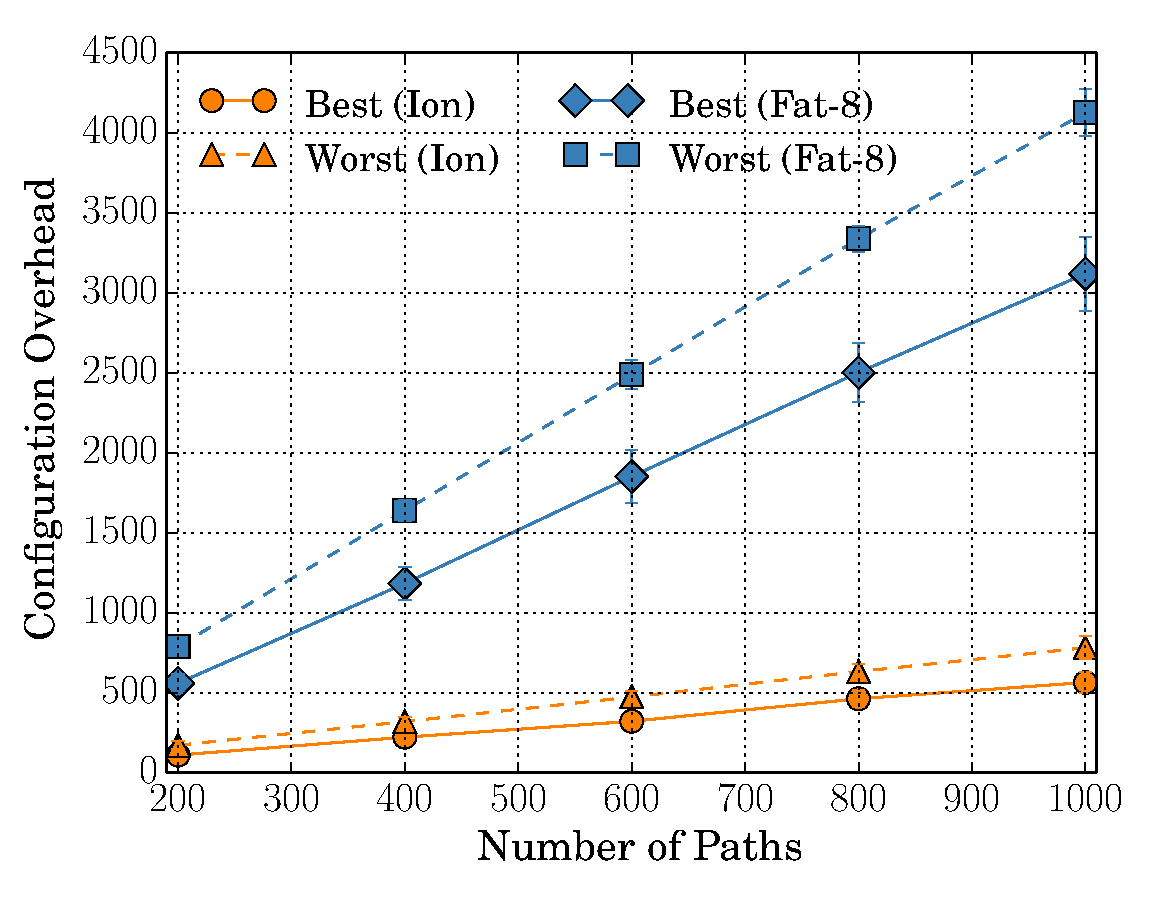
\includegraphics[width=0.7\columnwidth]{figures/confMCMC.eps}
	\compactcaption{MCMC Lines of Conf}
	\label{fig:confmcmc}
\end{figure}

\begin{figure}[t]
	\centering
	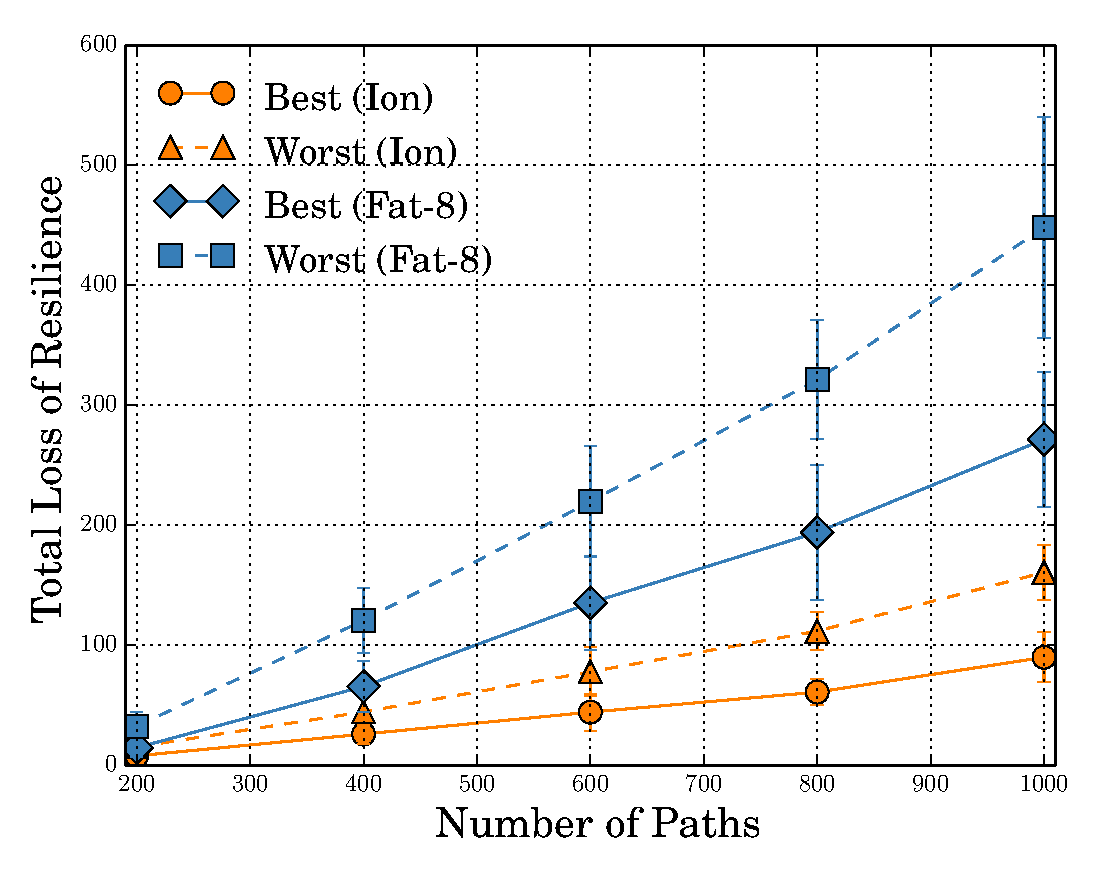
\includegraphics[width=0.7\columnwidth]{figures/TRLMCMC.eps}
	\compactcaption{MCMC TRL}
	\label{fig:trlmcmc}
\end{figure}



\section{Evaluation}
\section{Related \& Future Work} \label{sec:relatedwork}
\textbf{One Big Switch:} Kang et. al~\cite{oneswitch} tackle a 
similar problem of flow policy
enforcement. However, their end-point policies deal with simple
reachability. Their rule placement algorithm takes the path of the
flow in the network (called the routing policy) as an input. %  and place rules
% on this path to enforce the endpoint policy and taking in
% consideration switch table constraints
% Our solution can support enforcement of policies which
% require different routing policies.
Zhang et. al~\cite{distfirewall} build on the "one big switch"  
abstraction~\cite{oneswitch} to optimize for the specific case of
distributed firewall policy enforcement using ILP.  PGA~\cite{pga} provides
a graph-level abstraction for specifying network policies like ACLs and
middlebox service chaining. However, PGA abstracts the underlying
network as "one big switch" and cannot be used to compose policies like
tenant isolation or traffic engineering.
\begin{figure}[t]
	\centering
	\includegraphics[width=0.7\columnwidth]{figures/dcSynthesis.eps}
	\compactcaption{CDF for speedup achieved by divide-and-conquer synthesis.}
	\label{fig:dcsyn-cdf}
\end{figure}

 \noindent {\bf Controller synthesis:}
 Program synthesis has
 seen limited applications to SDN controllers~\cite{netegg,decentralize}.
These systems synthesize the
 behavior of individual switches (e.g., learning switches or
 firewalls); furthermore, these techniques apply to networks
 operating in a reactive mode (where the first packet of a connection
 is processed by the controller to determine the actions to
 employ). Such switch-centric approaches are too constraining and
 cannot be applied to realize network-wide objectives considered 
 in \name.
 Synthesis has been also used for generating consistent network
 updates~\cite{updates, customconsistency}. But this problem is orthogonal to 
 policy enforcement.
 
\noindent {\bf Policy languages:}
The closest approaches to ours are Merlin~\cite{merlin},
NetGen~\cite{netgen} and NetKAT~\cite{netkat}.  
In Merlin, data planes that adhere to policies
expressed using regular expressions are synthesized by first
intersecting the topology with the regular expressions appearing in
the policies and then encoding reachability in the intersected graph
using mixed integer linear programming (ILP).
%Unlike \Name, 
Merlin supports minimum and maximum bandwidth guarantees.
In its current iteration, 
Merlin's encoding does not support isolation policies, but we believe
that it could be extended to support them.  
%We cannot evaluate the
%performance impact of this extension, however.  
A more prominent
difference arises with unordered waypoint policies: expressing a
policy including a waypoint set $W$ of size $k$ requires a regular
expression of size exponential in $k$ as all the possible permutations
of the elements of $W$ must be considered. This fact clearly 
impacts the performance of 
Merlin's compiler that would have to generate a mixed ILP with a
large number of variables.  In \Name, this is not the case as waypoints
can be encoded with polynomially many constraints.  While this does
not affect the theoretical complexity, our compiler does not incur
an a-priori exponential blow-up; it rather relies on the power
of SMT solvers to guide the search.  This is one of the main aspects
behind our decision of not using regular expressions to express
policies.  \Name uses a restricted form of regular expressions as 
tactics that leverage the network topology.  While in Merlin,
regular expressions \emph{increase} the number of constraints
generated by the compiler, tactics \emph{decrease}
the number of generated constraints, therefore speeding up the search.
To the best of our knowledge, this is the first use of constraints
that leverages the topology structure to simplify the search.

In NetGen, network updates that adhere to policies expressed using
regular expressions are synthesized using SMT solvers.  Given a
specification which mentions the packet classes, the old path, and the
new path, NetGen solves the network change problem using an SMT solver.
Due to the use of regular expressions NetGen also suffers the
limitations we just discussed for Merlin.  Interestingly, NetGen uses
a specific encoding of regular expressions based on uninterpreted
functions that helps reduce the number of constraints. While this
encoding is fast when updating a single path, we do not see a way to
extend it to our global synthesis setting.  A crucial aspect of NetGen
is that in its problem formulation each path can be synthesized
independently and without affecting the other already synthesized
paths.  This is not the case when supporting isolation policies: if an
old path needs to be moved to satisfy a new policy (e.g., because a
link is under maintenance), re-synthesizing such a path can require
re-synthesizing other paths. 

NetKAT is a domain-specific language and logic for 
specifying and verifying network packet-processing functions
for SDN, based on Kleene algebra with tests (KAT). Semantically,
a NetKAT predicate and policy is a function that takes a packet
history and produces a set of packet histories, and can be used
to express certain network-wide policies like reachability 
and waypoints using regular expressions for describing the paths, 
and programs on virtual topologies which are translated to local
switch programs using BDDs and symbolic automata
~\cite{netkatcompiler}. However, their semantics
cannot be used to express policies based on hyperproperties
~\cite{hyperproperties}, i.e., 
the packet processing function requires multiple packet histories
as input. Traffic engineering or isolated paths are policies
based on hyperproperties. 
% \loris{we can have a small example of  this in appendix.}
\begin{figure}[t]
	\centering
	\includegraphics[width=0.65\columnwidth]{figures/linkTopology.eps}
	\compactcaption{Average synthesis time per packet class versus topology size for isolation workloads 
		with the ratio of packet classes to number of edge-aggregate links 0.25 and 10 low bandwidth links in the topology 
		have capacity policies.}
	\label{fig:link-capacity}
\end{figure}
% \noindent
% {\bf Synthesis for SDN:}
% Program synthesis has been actively applied in SDN for synthesizing the controller. Padon et. al in \cite{decentralize} try to synthesize
% local forwarding rules for a single switch based on a reactive
% forwarding policy.  NetEgg \cite{netegg} synthesizes the forwarding
% policy of a switch using examples of how the switch should function
% when it receives packets. These works deal with synthesis of
% forwarding behaviour of switches, and cannot be extended to satisfy
% network-wide policies.

% Write about PGA, NetGen, and efficient update synthesis.

\noindent
{\bf Future directions:}  
Fine-grained traffic engineering based on online demand/flow size estimation and 
rapid rerouting is also crucial for datacenter workloads, and extending \name's
TE policies to fine-grained timescales is subject of future work.
Also, the performance
of SMT solvers with optimization objectives is quite slow, and calls for 
domain-specific techniques to speed up the synthesis. Also, datacenter
networks are highly symmetrical, and this symmetry can be leveraged
to speed up synthesis (similar to the work of Plotkin et. al~\cite{symmetry} to
speed up network verification using symmetry). The main challenges of
using symmetry in synthesis is considering two aspects of symmetry: network
symmetry and policy symmetry. Also, our treatment of resilience synthesis
is preliminary and future work will be geared towards synthesizing resilient
forwarding planes incorporating capacity constraints and traffic engineering.
 

%!TEX root = paper.tex
\section{Conclusion}
We presented \name, a system for automatically synthesizing 
highly-resilient distributed hierarchical control planes---i.e., OSPF and 
BGP router configurations---from
high-level policies. For hierarchical control planes, 
we devised algorithms based on our OSPF-BGP interaction model. In 
practice, there exists hierarchical models, we can integrate these routing
models into \name's modular two-phase approach.
Similarly, we can modify OSPF synthesis to incorporate multi-path routing
for load-balancing etc. Finally, resilience is an important requirement, 
and extending \name to support other notions of policy-resilience
for $k > 1$ link failures is subject for future work.



%\bibliography{references}{}
%\bibliographystyle{acm}
 \appendix
 
\section{NP-completeness Proof of Enforcing Isolation Policies} \label{sec:isolationNP}
 We show that the graph 3-coloring problem, which is NP-complete reduces to the enforcement problem for
 reachability and isolation policies. The latter is also in NP, so after the reduction we 
 can conclude that it is also NP-complete.

Let $G=(V,E)$ be an instance of the graph 3-coloring problem.
The graph $G$ admits a 3-coloring if there exists a function 
$f:G\mapsto \{R,G,B\}$ such that for every edge $(v1,v2)\in E$,
$f(v_1)\neq f(v_2)$.

We now show how to construct a topology $T=(S,L)$ and a corresponding set of policies $P$ that can be 
enforced iff $G$ admits 3-coloring.
The topology $T$ is the one depicted in  \Cref{fig:swtopo}.
The set of flows is $V$, $v \in V$ we add a reachability policy $s >> d$ on the flow $v$.
For each edge $(v1,v2)\in E$ we add an isolation policy $v_1||v_2$.
% \begin{figure}[H] 
% 	\centering
% 	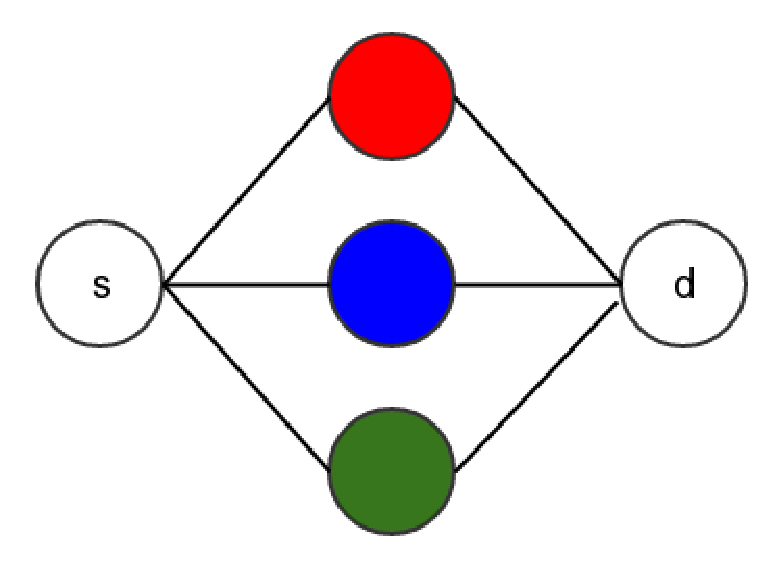
\includegraphics[width=0.5\columnwidth]{figures/color_topo.eps}
% 	\caption{The switch topology $T$. All circles represent switches and all reachability policies are $s$ to $d$}
% 	\label{fig:swtopo}
% \end{figure}
\begin{figure}[h!]
	\centering
	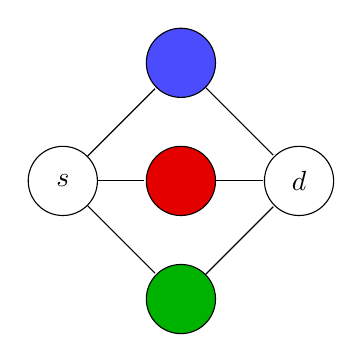
\begin{tikzpicture}[shorten >=0.5pt,node distance=1.5cm,on grid,auto] 
	\node[state] (s)   {$s$}; 
	\node[state, fill=black!10!red] (r) [right=of s] {}; 
	\node[state, fill=white!30!blue] (b) [above=of r] {};
	\node[state, fill=black!30!green] (g) [below=of r] {}; 
	\node[state] (d) [right=of r] {$d$}; 	
	\path[-] 
	(s) edge  node {} (r)
	edge node {} (b)
	edge node {} (g)
	(r) edge node {} (d)
	(g) edge node {} (d)
	(b) edge node {} (d);
	\end{tikzpicture}
	\caption{The switch topology $T$. All circles represent switches and all reachability policies are $s$ to $d$}
	\label{fig:swtopo}
\end{figure}
We now prove that if the policies can enforced then $G$ admits 3-coloring.
If the policy is enforced, we have a path from $s$ to $d$ for each flow/vertex $v$.
We can set $f(v)$ to the color of the corresponding middle-switch being crossed.
Since for every $(v1,v2)\in E$ the two flows for $v_1$ and $v_2$ cannot share any edge,
they must have crossed two middle-switches with different colors and $f$ is a correct 3-coloring.
The other direction of the proof is analogous.

 
% \subsection{Enforcement of Waypoint Policies}
% Given a undirected graph $G={V,E}$. Let us assume there exists an polynomial-time algorithm to compute the reachability paths satisfying the policies of the following types on the graph : \\
% \begin{itemize} 
% 	\item \textbf{P1} : $v_1 >> v_2 \Rightarrow$ There exists a path from $v_1$ to $v_2$ satisfying all input policies. A property of the path is that it does not have repeat a vertex (no forwarding loops).
% 	\item \textbf{P2} : $v_1 >> W >> v_2 \Rightarrow$ The path from $v_1$ to $v_2$  should pass through the vertices in the set $W$ in any order, without repeating a vertex.
% \end{itemize}
% \textbf{Reduction of Hamiltonian Cycle Problem} : Given a undirected graph $G={V,E}$, find $v \in V$ such that the degree of $v$ is the minimum in the graph (Will work for any vertex actually). If a Hamiltonian cycle is present in the graph, it will have the vertex $v$ in the cycle, and one of the edges from $v$.  \\
% Lets take a $n \in Neighbours(v)$. Let the input policies to our algorithm be : 
% \begin{itemize}
% 	\item \textbf{P4} : $v >> W >> n$ where $W = V - \{v,n\} $ 
% \end{itemize}
%P4 cimputes a simple path from $v$ to $n$ which passes through all the other vertices in the graph which is the Hamiltonian path problem. Since computing the Hamiltonian path is NP-hard, the problem of path computation for the waypoint policies as specified is NP-hard. 
\section{Tactics}
\begin{theorem}[Soundness]
	For a packet class $pc$, if the path $\pi \models_{pc} \Psi \wedge \Psi_R$, then $\pi \models R$.
\end{theorem}
\begin{proof}
	The proof of this theorem is by contradiction for each type of tactic. \newline
	\textbf{Type 1}: R = $\neg (l_{src} .^i .^* l_{dst})$ \\
	%$\forall sw,k \geq i + 1. (sw,pc,k) \notin Reach \implies \pi \models \neg (l_{src} .^i .^* l_{dst}) $ \newline
	\textbf{Assume  $\pi \not\models R$}.  $\pi \models l_{src} .^i .^* l_{dst}$. \\
	Thus, $\pi = src\ sw_1 \ldots sw_i \ldots dst$. \\
	Therefore,  $(dst, pc, k_{dst}) \in Reach, k_{dst} \geq i + 1$. \\
	However, $\pi \models_{pc} \Psi_R \Leftrightarrow \pi \models_{pc} \forall sw,k \geq i + 1. (sw,pc,k) \notin Reach$.
	Contradiction, as $\exists sw, k \geq i + 1. (sw,pc,k) \in Reach$.
	\newline
	\newline
	\textbf{Type 2}: $R = \neg (l_{src} .^i \ l \ .^* l_{dst})$ \newline
	\textbf{Assume  $\pi \not\models R$}. $\pi \models l_{src} .^i \ l \ .^* l_{dst}$. \\
	Thus, $\pi = src\ sw_1 \ldots sw_i \ sw_{i+1} \ldots dst$ such that $\phi(sw_{i+1}) = l$. Also $sw_{i+1} \not=dst$ (dst has to be the last switch in $\pi$)\\
	Therefore,  $(sw_{i+1}, pc, i+1) \in Reach$. \\
	However,
	$\pi \models_{pc} \Psi_R \Leftrightarrow \pi \models_{pc}\forall sw.~ \phi(sw) = l ~\wedge~ sw \not= dst \implies  (sw, pc, i + 1) \notin Reach$. \\
	Contradiction, as $\exists sw. ~ \phi(sw) = l ~\wedge~ sw \not= dst \wedge (sw,pc,i+1) \in Reach$.
	\newline \newline
	\textbf{Type 3}: $R = \neg (l_{src} .^i \ l_1 \ l_2 \ .^* l_{dst})$ \newline
	\textbf{Assume  $\pi \not\models R$}. $\pi \models l_{src} .^i \ l_1 \ l_2 \ .^* l_{dst}$. \\
	Thus, $\pi = src\ sw_1 \ldots sw_i \ sw_{i+1} \ sw_{i+2} \ldots dst$ such that $\phi(sw_{i+1}) = l_1, \phi(sw_{i+2}) = l_2$. Also $sw_{i+2} \not=dst$ (dst has to be the last switch in $\pi$)\\
	Therefore,  $(sw_{i+1}, pc, i+1) \in Reach \wedge (sw_{i+1}, sw_{i+2}, pc) \in Fwd$. \\
	However,
	$\pi \models_{pc} \Psi_R \Leftrightarrow \pi \models_{pc} \forall n_1, n_2.~\phi(n_1) = l_1~\wedge~ \phi(n_2) = l_2 ~\wedge~ n_2 \not=dst  \implies 
	\neg (Reach(n_1, pc, i + 1) \wedge Fwd(n_1, n_2, pc))$. \\
	Contradiction, as $\exists n_1. n_2. ~\phi(n_1) = l_1~\wedge~ \phi(n_2) = l_2 ~\wedge~ n_2 \not=dst \wedge Reach(n_1, pc, i + 1) \wedge Fwd(n_1, n_2, pc)$. 
\end{proof}
\begin{theorem}[Completeness]
	For a packet class $pc$, if the path $\pi \models_{pc} \Psi ~\wedge~ \pi \models R$, then $\pi \models_{pc} \Psi_R$.
\end{theorem}
\begin{proof}
	The proof of this theorem is by contradiction for each type of tactic. \newline
	\textbf{Type 1}: $R = \neg (l_{src} .^i .^* l_{dst})$ \newline
	\textbf{Assume  $\pi \not\models_{pc} \Psi_R$}. $\pi \not\models_{pc} \forall sw,k \geq i + 1. (sw,pc,k) \notin Reach$ \newline
	Therefore $\exists sw, k \geq i + 1. (sw,pc,k) \in Reach$. \\
	Therefore, $\pi \models l_{src}\ .^i \ .^* \ \phi(sw) \ .^* \ l_{dst} \implies \pi \models l_{src} .^i .^* l_{dst}$
	Contradiction, as $\pi \models R$.
	\newline 
	\newline 
	\textbf{Type 2}: $R = \neg (l_{src} .^i \ l \ .^* l_{dst})$ \newline
	\textbf{Assume  $\pi \not\models_{pc} \Psi_R$}.  $\pi \not\models_{pc}\forall sw.~ \phi(sw) = l ~\wedge~ sw \not= dst \implies  (sw, pc, i + 1) \notin Reach$. \\
	Therefore $\exists sw. \ sw \not= dst \ \wedge \ \phi(sw) = l \ \wedge \ (sw,pc,i+1) \in Reach$. \\
	Therefore, $\pi \models l_{src}\ .^i \ l \ .^* \ l_{dst}$. \\
	Contradiction, as $\pi \models R$. 
	\newline  
	\newline
	\textbf{Type 3}: $R = \neg (l_{src} .^i \ l_1 \ l_2 \ .^* l_{dst})$ \newline
	\textbf{Assume  $\pi \not\models_{pc} \Psi_R$}.  $\pi \not\models_{pc} \forall n_1, n_2.~\phi(n_1) = l_1~\wedge~ \phi(n_2) = l_2 ~\wedge~ n_2 \not=dst  \implies 
	\neg (Reach(n_1, pc, i + 1) \wedge Fwd(n_1, n_2, pc))$. 
	Therefore $\exists n_1, n_2. ~\phi(n_1) = l_1~\wedge~ \phi(n_2) = l_2 ~\wedge~ n_2 \not=dst ~\wedge~ Reach(n_1, pc, i + 1) ~\wedge~ Fwd(n_1, n_2, pc)$. \\
	Therefore, $\pi \models l_{src}\ .^i \ l_1~l_2 \ .^* \ l_{dst}$. \\
	Contradiction, as $\pi \models R$.
\end{proof}
%\section{Constraint Evaluation}
%\loris{This analysis can go in appendix}
%\kausik{Do we need this section? We can just have the table and the time taken to add these constraints in the evaluation section.}
%In the section, we evaluate the number of constraints required to add to the Z3 solver. Let $|S|$ be the number of switches in the topology, $|L|$ be the number of edges in the topology, $|PC|$ be the number of packet classes, $|I|$ be the number of traffic isolation policies and $\mu$ be the max path length. Let $deg$ be the maximum number of neighbours for a switch (degree of the topology).
%
%We encode the forwarding set constraint (\cref{eq:fwdset}) using a SAT encoding rather than an SMT encoding for better performance. To express the constraint that the count of forwarding rules is not more than one, we can do this by adding an $or$ of clauses, where each clause is an $and$ of one rule set to true and all others set to false.
%\loris{why the Z3 syntax? use the same as before.
%Also, there is a verbatim environment that would simplify your life with latex. begin {verbatim}... end {verbatim} }
%An example for switch s and neighbours \{t,u\} is \newline
%\verb|(or| \\
%\hspace*{10pt}\verb|(and Fwd(s, t, pc)|  \verb|(not Fwd(s, u, pc)))| \\
%\hspace*{10pt}\verb|(and Fwd(s, u, pc)|  \verb|(not Fwd(s, t, pc)))| \\
%\hspace*{10pt}\verb|(and (not Fwd(s, u, pc))|  \verb|(not Fwd(s, t, pc)))|\\
%\verb|)| 
%
%Thus, the number of terms in a forwarding rule constraint for a switch and packet class is $deg \times (deg+1)$. We add a single \verb|or| constraint for each switch and packet class in the network. Therefore, the count of constraints is $|S| \times |PC|$.
%
%\loris{this need to be measured, please run an experiment in which you measure exactly
%the cost of adding the constraints vs cost of calling solve}
%The major bulk of time is consumed by the creation of the constraints for backward propagation of reachability (\cref{eq:bckprop}). The number of constraints added to the solver is $|S| \times |PC| \times \mu$. We are using a quantifier-free encoding for better performance, so expressing the $exists$ is done by a $or$ clause of the set of neighbours for a switch. Therefore, the size of each constraint is $deg$. 
%
%For each traffic isolation policy, we need to add constraints for each edge of the network, so that the two packet classes dont share the edge. Therefore, the number of constraints added is $|L| \times |I|$ and the size of each constraint is constant size of two terms.
%
%\begin{table}[H]
%\begin{center}
%	\begin{tabular}{||m{6em} | m{7em} | m{7em} ||} 
%		\hline
%		Constraints & Number & Size \\ [0.5ex] 
%		\hline\hline
%		Forwarding Rules & $|S| \times |PC| $ & $deg \times (deg + 1)$ \\ [0.5ex] 
%		\hline
%		Reachability Propagations & $|S| \times |PC| \times \mu $ & $deg$ \\ [0.5ex] 
%		\hline
%		Isolation & $|L| \times |I|$ & 2 \\
%		\hline
%	\end{tabular}
%\end{center}
%\caption{Number and Size of Constraints} \label{tab:title} 
%\end{table}
\bibliographystyle{abbrv}
\begin{small}
	\bibliography{references}
\end{small}
\end{document}
